\input templates/header

\usepackage{epigraph}
\usepackage[normalem]{ulem}
\usepackage{xcolor}
\usepackage{colortbl}
\usepackage{tikz}
\usepackage[normalem]{ulem}
\usepackage[absolute,overlay]{textpos}
\usetikzlibrary{trees}
\usetikzlibrary{shapes}
\usetikzlibrary{positioning}

\setlength{\epigraphwidth}{6cm}

\usepackage{xmpmulti}
\usepackage{listings}

\lstset{
  basicstyle=\ttfamily,
%  columns=fullflexible,
  keywordstyle=\color{red}\bfseries,
  commentstyle=\color{blue},
  showstringspaces=false,
  escapeinside={<@}{@>},
}

\newcommand*\circled[1]{\tikz[baseline=(char.base)]{
      \node[circle,ball color=blue, shade, 
 color=white,inner sep=1.2pt] (char) {\tiny #1};}}


\title[ASD - Programmazione Dinamica]{\textbf{Algoritmi e Strutture Dati}\\[24pt]Programmazione dinamica -- Parte 1}

\graphicspath{{figs/13/}}

\begin{document}



%-------------------------------------------------------------------------
\FrameTitle{}

%-------------------------------------------------------------------------
\FrameContent


%%%%%%%%%%%%%%%%%%%%%%%%%%%%%%%%%%%%%%%%%%%%%%%%%%%%%%%%%%%%%%%%%%%%%%%%%%
\section{Introduzione}
%%%%%%%%%%%%%%%%%%%%%%%%%%%%%%%%%%%%%%%%%%%%%%%%%%%%%%%%%%%%%%%%%%%%%%%%%%

\begin{frame}{Tecniche di soluzione problemi}

\BIL
\item Divide-et-impera 
\item Programmazione dinamica / memoization
\item Tecnica greedy
\item Ricerca locale 
\item Backtrack
\item Algoritmi probabilistici
\item Tecniche di approssimazione
\EIL

\end{frame}

\begin{frame}{Programmazione dinamica in pillole}

\BIL
\item Un metodo per spezzare un problema ricorsivamente in sottoproblemi
\item Ogni sottoproblema viene risolto una volta sola
\item La sua soluzione viene memorizzata in una tabella
\item Nel caso un sottoproblema debba essere risolto nuovamente, si ottiene la
  sua soluzione dalla tabella
\item La tabella è facilmente indirizzabile (lookup in $O(1)$)
\EIL
    
\epigraph{\alert{Those who cannot remember the past are condemned to repeat it}
}{\textit{George Santayana, 1905}}

\end{frame}


% \begin{frame}{Quale tecnica applicare?}
%
% \BB{Sottostruttura ottima}
% E' possibile spezzare ricorsivamente un problema in sottoproblemi più piccoli? Le decisioni prese per risolvere un problema rimangono valide quando esso diviene un sottoproblema di un problema più grande?
%
% \begin{columns}[T]
% \column{0.45\textwidth}
% \BB{Risposta: S\`I}
% \BIL
% \item Divide-et-impera
% \item \alert{Programmazione dinamica}
% \item \alert{Memoization}
% \item Greedy
% \item Backtrack
% \EIL
% \column{0.45\textwidth}
% \BB{Risposta: NO}
% \BIL
% \item Backtrack
% \item Oppure, risoluzione ad-hoc
% \EIL
% \end{columns}
%
% \end{frame}
%
% \begin{frame}{Quale tecnica applicare?}
%
% \BB{Spazio dei sottoproblemi}
% Lo spazio dei sottoproblemi ha dimensione superpolinomiale?
%
% \bigskip
% \begin{columns}[T]
%
% \column{0.45\textwidth}
% \BB{Risposta: S\`I}
% \BIL
% \item Backtrack
% \EIL
%
% \column{0.45\textwidth}
% \BB{Risposta: NO}
% \BIL
% \item Divide-et-impera
% \item \alert{Programmazione dinamica}
% \item \alert{Memoization}
% \item Greedy
% \EIL
%
% \end{columns}
%
% \end{frame}
%
%
% \begin{frame}{Quale tecnica applicare?}
%
% \BB{Ripetizioni}
% Lo stesso sottoproblema può occorrere più volte come sottoproblema di un problema più grande?
%
% \bigskip
% \begin{columns}[T]
% \column{0.45\textwidth}
% \BB{Risposta: S\`I}
% \BIL
% \item \alert{Programmazione dinamica}
% \item \alert{Memoization}
% \item Greedy
% \EIL
% \column{0.45\textwidth}
% \BB{Risposta: NO}
% \BIL
% \item Divide-et-impera
% \item Greedy
% \EIL
% \end{columns}
%
% \end{frame}
%
% \begin{frame}{Quale tecnica applicare?}
%
% \BB{Copertura dei sottoproblemi}
% \BIL
% \item Per risolvere il problema principale, è necessario risolvere tutti i sottoproblemi?
% \EIL
%
% \bigskip
% \begin{columns}[T]
% \column{0.45\textwidth}
% \BB{Risposta: S\`I}
% \BIL
% \item \alert{Programmazione dinamica}
% \item \alert{Memoization}
% \EIL
% \column{0.45\textwidth}
% \BB{Risposta: NO}
% \BIL
% \item Greedy
% \item \alert{Memoization}
% \EIL
% \end{columns}
%
% \end{frame}


\begin{frame}{Approccio generale}

\vspace{-9pt}
\IG{1.0}{progrdyn.pdf}

\end{frame}

\begin{frame}{Un po' di storia}

\BIL
\item Il termine \alert{Dynamic Programming} è stato coniato da Richard Bellman 
agli inizi degli anni '50, nell'ambito dell'ottimizzazione matematica   
\item Inizialmente, si riferiva al processo di risolvere un problema compiendo
le migliori decisioni una dopo l'altra.
\item "Dynamic" doveva dare un senso "temporale"
\item "Programming" si riferiva all'idea di creare "programmazioni ottime",
per esempio nel campo della logistica
\EIL

\bigskip
\url{https://en.wikipedia.org/wiki/Dynamic_programming\#History}

\end{frame}



%%%%%%%%%%%%%%%%%%%%%%%%%%%%%%%%%%%%%%%%%%%%%%%%%%%%%%%%%%%%%%%%%%%%%%%%%%
\section{Domino}
%%%%%%%%%%%%%%%%%%%%%%%%%%%%%%%%%%%%%%%%%%%%%%%%%%%%%%%%%%%%%%%%%%%%%%%%%%

\begin{frame}{Problema 1 -- Domino lineare}

\vspace{-9pt}
\begin{myboxtitle}[Definizione]
Il gioco del domino è basato su tessere di dimensione $2 \times 1$. Scrivere
un algoritmo efficiente che prenda in input un intero $n$ e restituisca il numero di possibili disposizioni di $n$ tessere in un rettangolo $2 \times n$.
\end{myboxtitle}

\bigskip
\BB{Esempio}

I casi (a)-(e) della figura rappresentano le cinque disposizioni possibili con cui è possibile riempire un rettangolo $2 \times 4$. 

\begin{center}
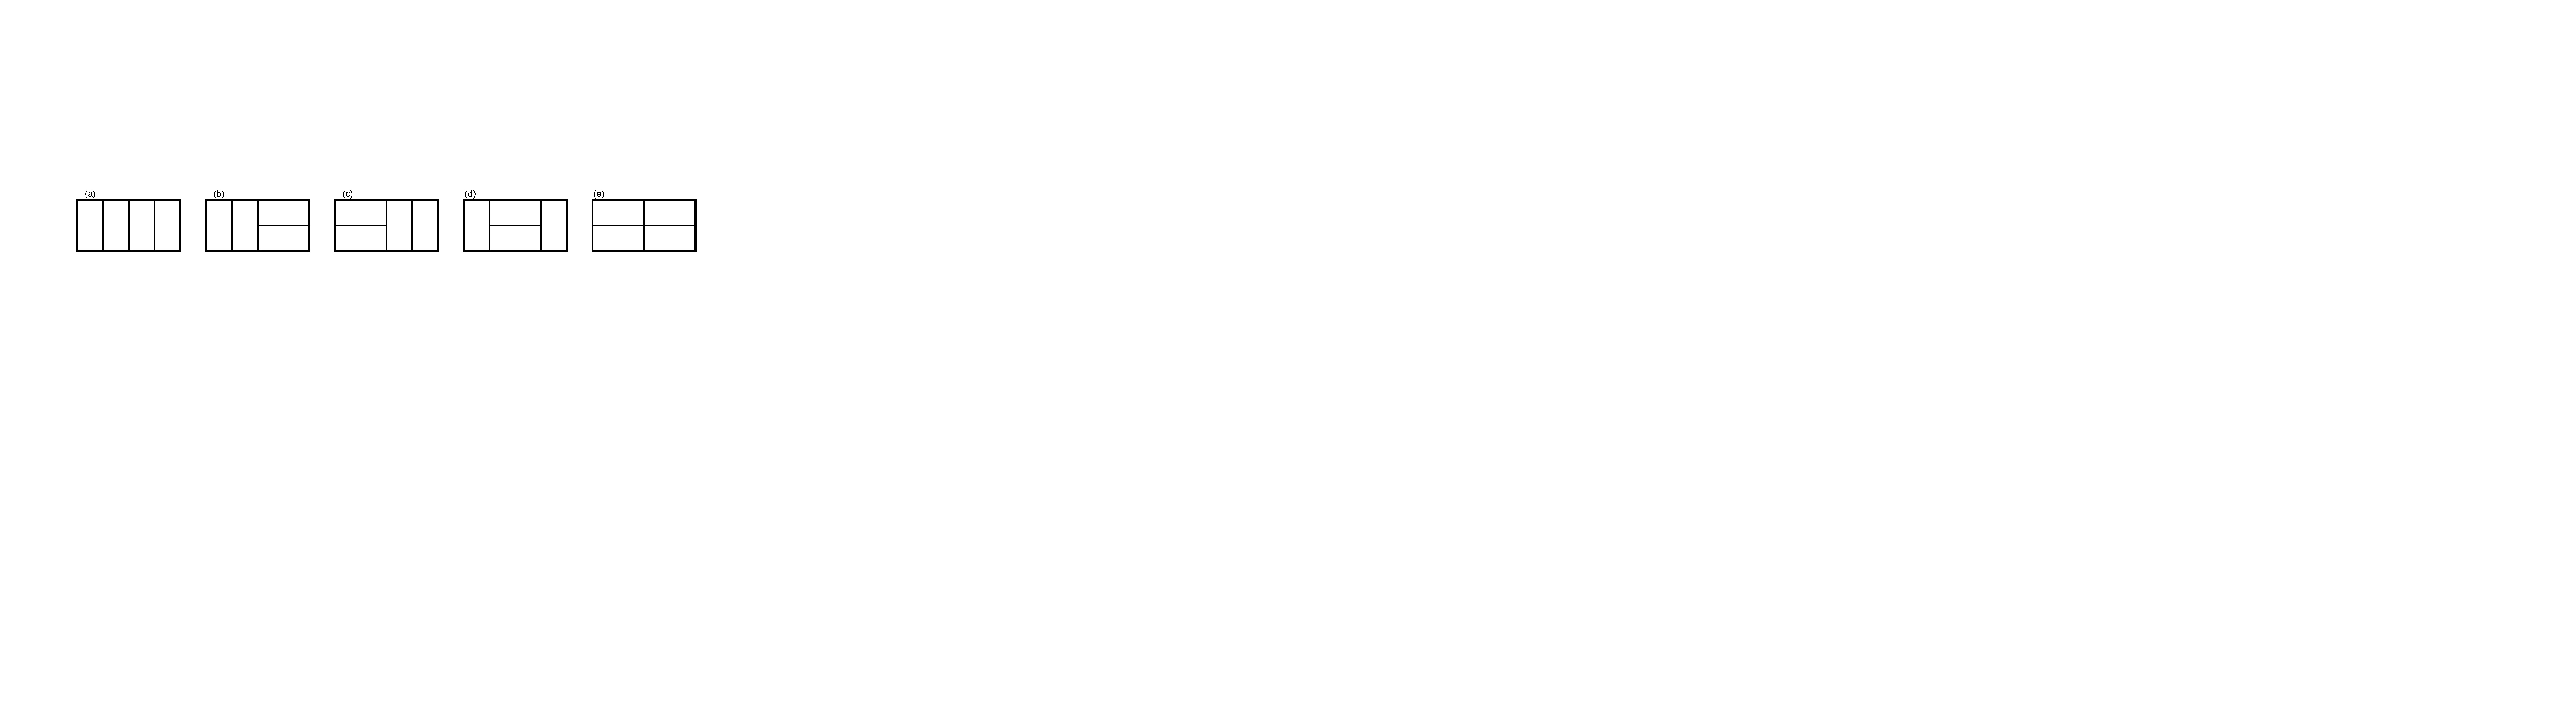
\includegraphics[width=1.0\textwidth]{domino.pdf}
\end{center}

\end{frame}


%-------------------------------------------------------------------------
\begin{frame}<1|handout:0>[fragile]{Domino}

\vspace{-9pt}
\BB{Come risolvereste il problema?}

\end{frame}

%-------------------------------------------------------------------------
\begin{frame}{Domino}

\vspace{-9pt}
\begin{myboxtitle}[Definizione ricorrenza]
Definiamo una formula ricorsiva $DP(n)$ che ci permetta di calcolare il numero di disposizioni possibili quando si hanno $n$ tessere.
\end{myboxtitle}

\begin{overprint}
\onslide<1|handout:0>
\BIL
\item Quante disposizioni possibili se non ho tessere ($n=0$)?
\item Quante disposizioni possibili se ho solo una tessera ($n=1$)?
\EIL
\onslide<2|handout:1>
\BIL
\item Con $n=0$, esiste una sola disposizione possibile (nessuna tessera)
\item Con $n=1$, esiste una sola disposizione possibile (tessera verticale)
\EIL
\onslide<3|handout:0>
\BIL
\item Cosa succede se decido di mettere l'ultima tessera in verticale?
\item Cosa succede se decido di mettere l'ultima tessera in orizzontale?
\EI
\onslide<4|handout:2>
\BIL
\item Se metto una tessera in verticale, risolverò il problema
di dimensione $n-1$
\item Se metto una tessera in orizzontale, ne devo mettere due; risolverò
il problema di dimensione $n-2$
\EIL
\end{overprint}

\bigskip
\begin{overprint}
\onslide<1|handout:0>
\[
DP(n) = \begin{cases}
  ? & n \leq 1 \\
  \makebox[3.5cm][l]{?} & n>1
\end{cases}
\]
\onslide<2-3|handout:1>
\[
DP(n) = \begin{cases}
  1 & n \leq 1 \\
  \makebox[3.5cm][l]{?} & n>1
\end{cases}
\]
\onslide<4|handout:2>
\[
DP(n) = \begin{cases}
  1 & n \leq 1 \\
  DP(n-2)+DP(n-1) & n>1
\end{cases}
\]
\end{overprint}

\end{frame}

\begin{frame}<1|handout:0>[fragile]{Serie matematica}

\vspace{-9pt}
\BB{La serie generata è la seguente}

\begin{lstlisting}
1, 1, 2, 3, 5, 8, 13, 21, 34, 55, 89, ...
\end{lstlisting}

\BB{Ricorda niente?}

\end{frame}


\begin{frame}[fragile]{Serie matematica}

\vspace{-9pt}
\BB{La serie generata è la seguente}

\begin{lstlisting}
1, 1, 2, 3, 5, 8, 13, 
21, 34, 55, 89, ...
\end{lstlisting}

\begin{textblock*}{5cm}(7.6cm,0.6cm) % {block width} (coords)
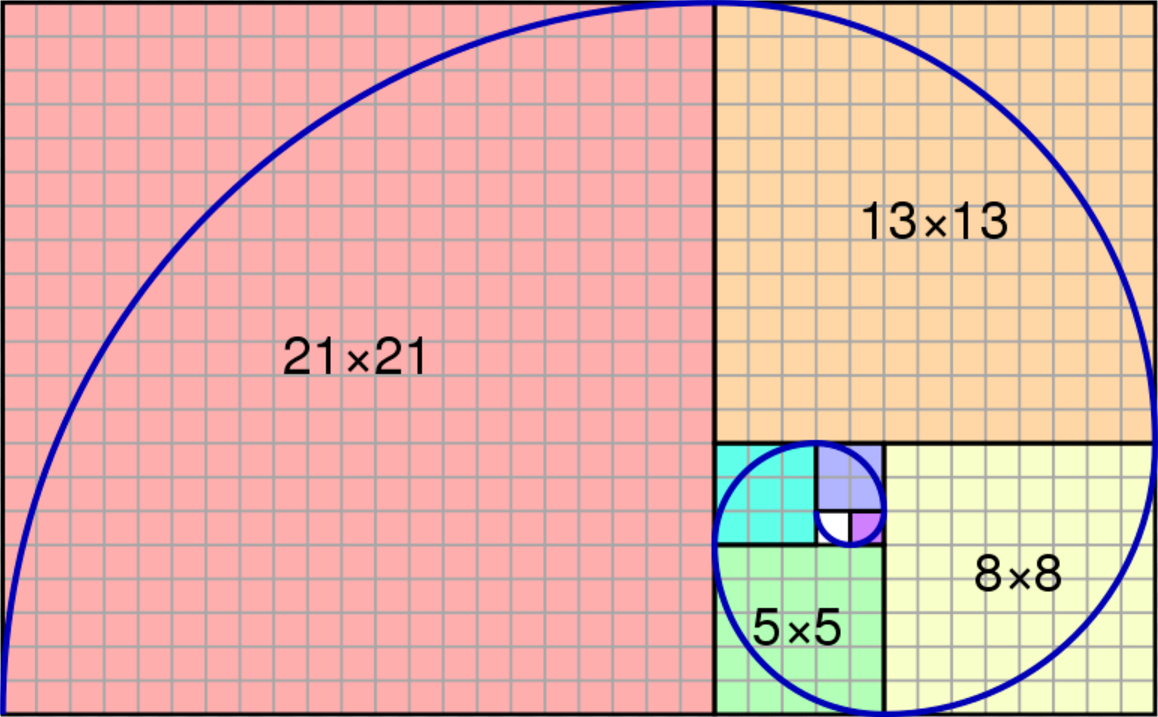
\includegraphics[width=5cm]{fibonacci.png}
\end{textblock*}

\begin{myboxtitle}[Successione di Fibonacci]
$DP(n)$ è pari al $n+1$-esimo numero della serie di Fibonacci, introdotta da Leonardo Pisano detto il Fi'Bonacci (1175--1235).
\end{myboxtitle}

\BIL
\item Definiti per descrivere la crescita di una popolazione di conigli (!)
\item In natura: Pigne, conchiglie, parte centrale dei girasoli, etc.
\item In informatica: Alberi AVL minimi, Heap di Fibonacci, etc.
\EIL

\end{frame}


\begin{frame}[fragile]{Domino - Algoritmo ricorsivo}

\vspace{-9pt}
\BB{Algoritmo ricorsivo che risolve il problema Domino}

\begin{Procedure}
\caption[A]{\INTEGER\ \textsf{domino1}(\INTEGER\ $n$)}
  \eIf{$n \leq 1$}{
    \Return $1$\;
  }{
    \Return $\textsf{domino1}(n-1) + \textsf{domino1}(n-2)$\;
  }
\end{Procedure}

\BB{Qual è l'equazione di ricorrenza associata a \textsf{domino1()}?}

\end{frame}

\begin{frame}{Complessità computazionale}

\vspace{-9pt}
\BB{Equazione di ricorrenza associata a \textsf{domino1()}}

\[
  T(n) = \begin{cases}
  1 & n \leq 1 \\
  T(n-1)+T(n-2)+1 & n > 1\\
  \end{cases}
\]

\BB{Qual è la complessità di \textsf{domino1()}?}

Ricorrenza lineare di ordine costante:
\BI
\item $a_1 = 1, a_2=1, a= a_1+a_2 = 2, \beta=0$
\item Complessità: $\Theta(a^n \cdot n^\beta)$
\EI

\[
T(n) = \Theta(2^n)
\]

\end{frame}

%-------------------------------------------------------------------------
\begin{frame}{Albero di ricorsione di \textsf{domino1()}}
  
\IG{1.0}{fibonacci-tree.pdf}

Molti sotto-problemi ripetuti!
\end{frame}

%-------------------------------------------------------------------------
\begin{frame}{Come evitare di risolvere un problema più di una volta}
  
\BB{Tabella DP}
\BIL
\item Quando risolviamo un problema, memorizziamo il risultato che otteniamo
in una \alert{tabella $DP$} (vettore, matrice, dizionario, etc)
\item La tabella deve contenere un elemento per ogni sottoproblema che dobbiamo risolvere
\EIL

\smallskip
\BB{Casi base}
\BIL
\item Memorizziamo i casi base direttamente nelle posizioni relative
\EIL

\smallskip
\BB{Iterazione bottom-up}
\BIL
\item Si parte da quelli che possono essere risolti a partire dai
casi base
\item Si sale verso problemi via via più grandi ...
\item ... fino a raggiungere il problema originale
\EIL

\end{frame}



%-------------------------------------------------------------------------
\begin{frame}[fragile]{Domino: algoritmo iterativo}

\vspace{-9pt}
\BB{Algoritmo iterativo che risolve il problema Domino}

\begin{Procedure}
\caption[A]{\INTEGER\ \textsf{domino2}(\INTEGER $n$)}
  $DP = \NEW\ \INTEGER[0 \ldots n]$\;
  $DP[0] = DP[1] = 1$\;
  \For{$i = 2$ \TO\ $n$}{
    $DP[i] = DP[i-1] + DP[i-2]$\;
  }
  \Return $DP[n]$\;
\end{Procedure}

\begin{center}
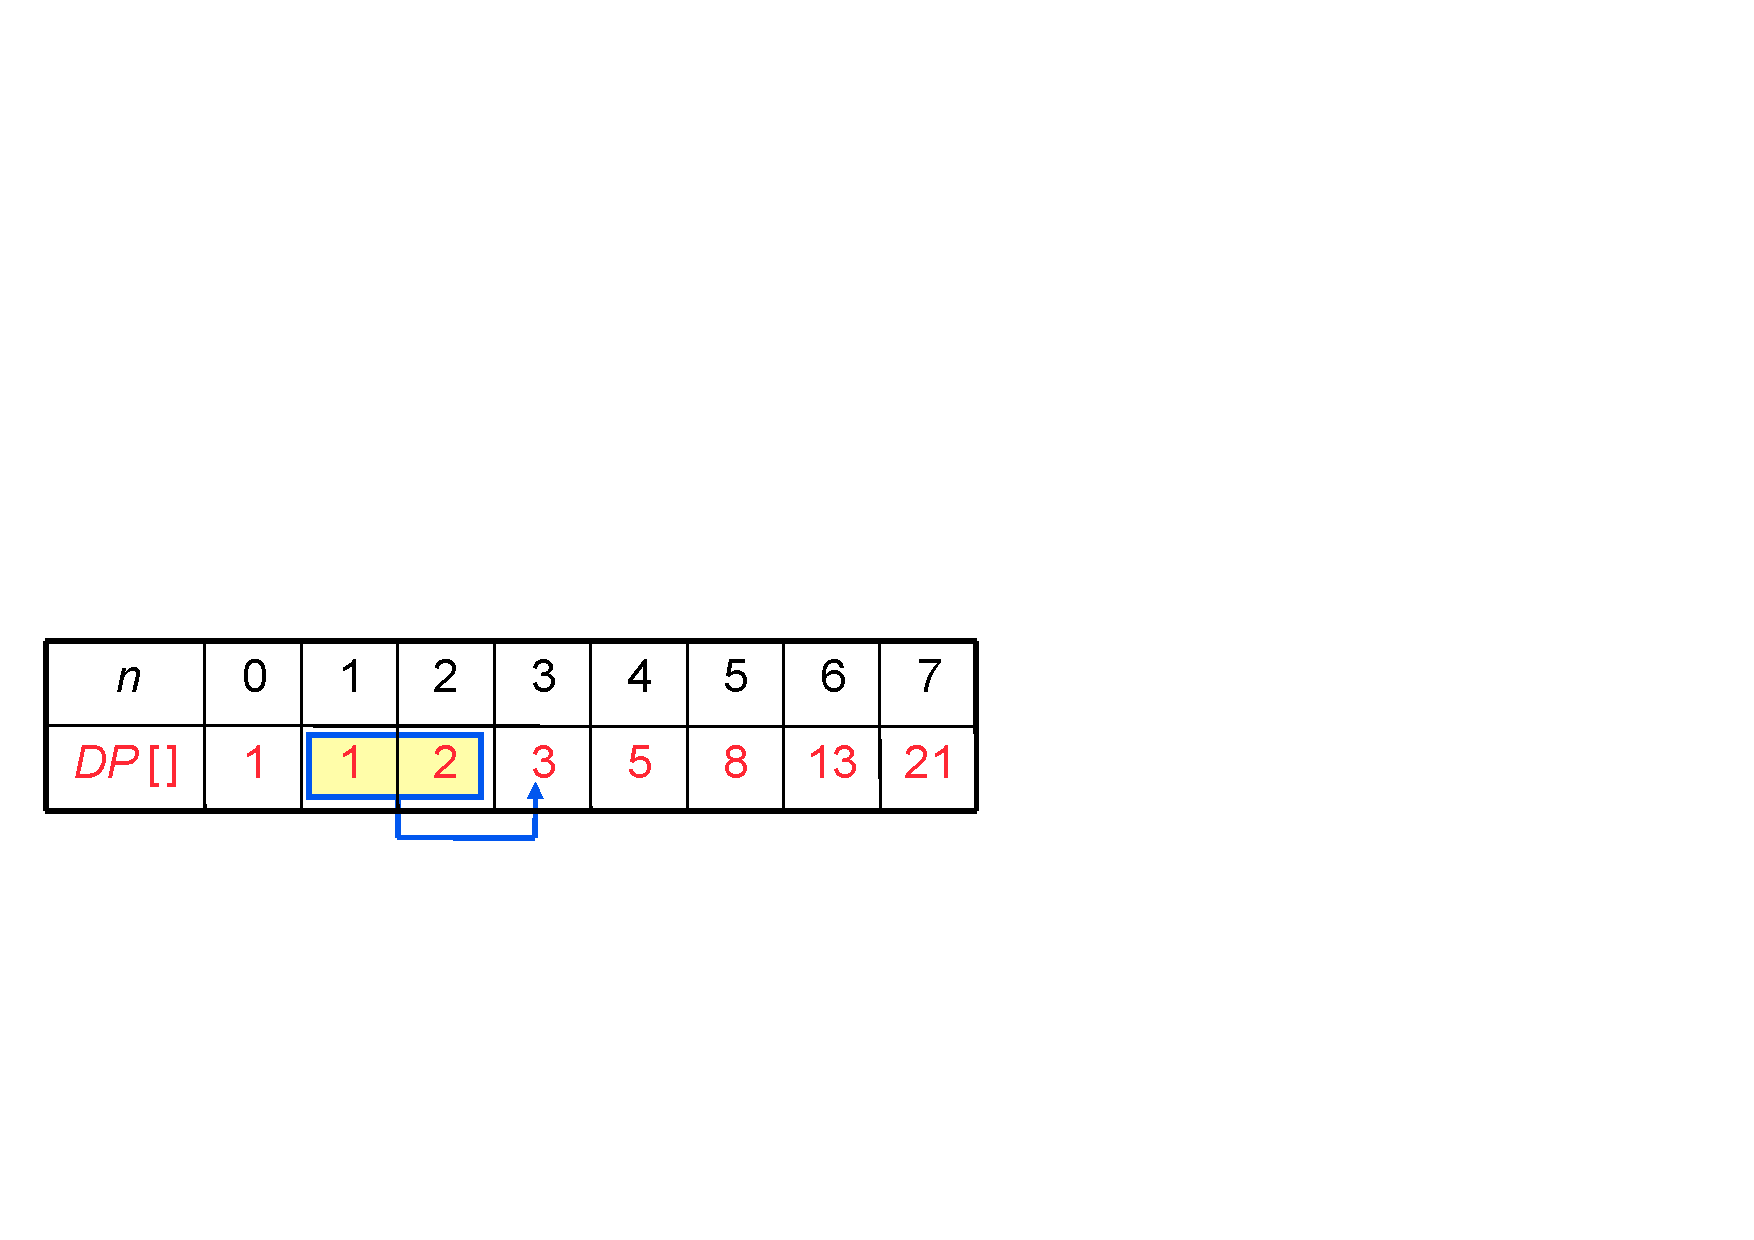
\includegraphics[width=0.75\textwidth]{fib-table1.pdf}
\end{center}

\end{frame}



%-------------------------------------------------------------------------
\begin{frame}[fragile]{Domino}

\begin{Procedure}
\caption[A]{\INTEGER\  \textsf{domino2}(\INTEGER $n$)}
  $DP = \NEW\ \INTEGER[0 \ldots n]$\;
  $DP[0] = DP[1] = 1$\;
  \For{$i = 2$ \TO\ $n$}{
    $DP[i] = DP[i-1] + DP[i-2]$\;
  }
  \Return $DP[n]$\;
\end{Procedure}

\begin{columns}[T]
\column{0.72\textwidth}
\BB{Qual è la complessità in \alert{tempo} di $\textsf{domino2}(n)$?}
\pause
\column{0.27\textwidth}
\bigskip
\alert{$T(n) = \Theta(n)$}
\end{columns}

\begin{columns}[T]
\column{0.72\textwidth}
\BB{Qual è la complessità in \alert{spazio} di $\textsf{domino2}(n)$?}
\pause
\column{0.27\textwidth}
\bigskip
\alert{$S(n) = \Theta(n)$}
\end{columns}

\begin{columns}[T]
\column{0.72\textwidth}
\BB{Possiamo fare \alert{"meglio di così"}?}
\pause
\column{0.27\textwidth}
\bigskip
\alert{Possiamo ridurre lo spazio utilizzato}
\end{columns}

\end{frame}

%-------------------------------------------------------------------------
\begin{frame}[fragile]{Domino}

\begin{columns}[T]
\column{0.38\textwidth}
\vspace{-8pt}
\begin{Procedure}
\caption[A]{\INTEGER\ \textsf{domino3}(\INTEGER\ $n$)}
  $\INTEGER\ \mathit{DP_0} = 1$\;
  $\INTEGER\ \mathit{DP_1} = 1$\;
  $\INTEGER\ \mathit{DP_2} = 1$\;
  \For{$i = 2$ \TO\ $n$}{
    $\mathit{DP_0} = \mathit{DP_1}$\;
    $\mathit{DP_1} = \mathit{DP_2}$\;
    $\mathit{DP_2} = \mathit{DP_0} + \mathit{DP_1}$\;
  }
  \Return $DP_2$\;
\end{Procedure}
\column{0.62\textwidth}

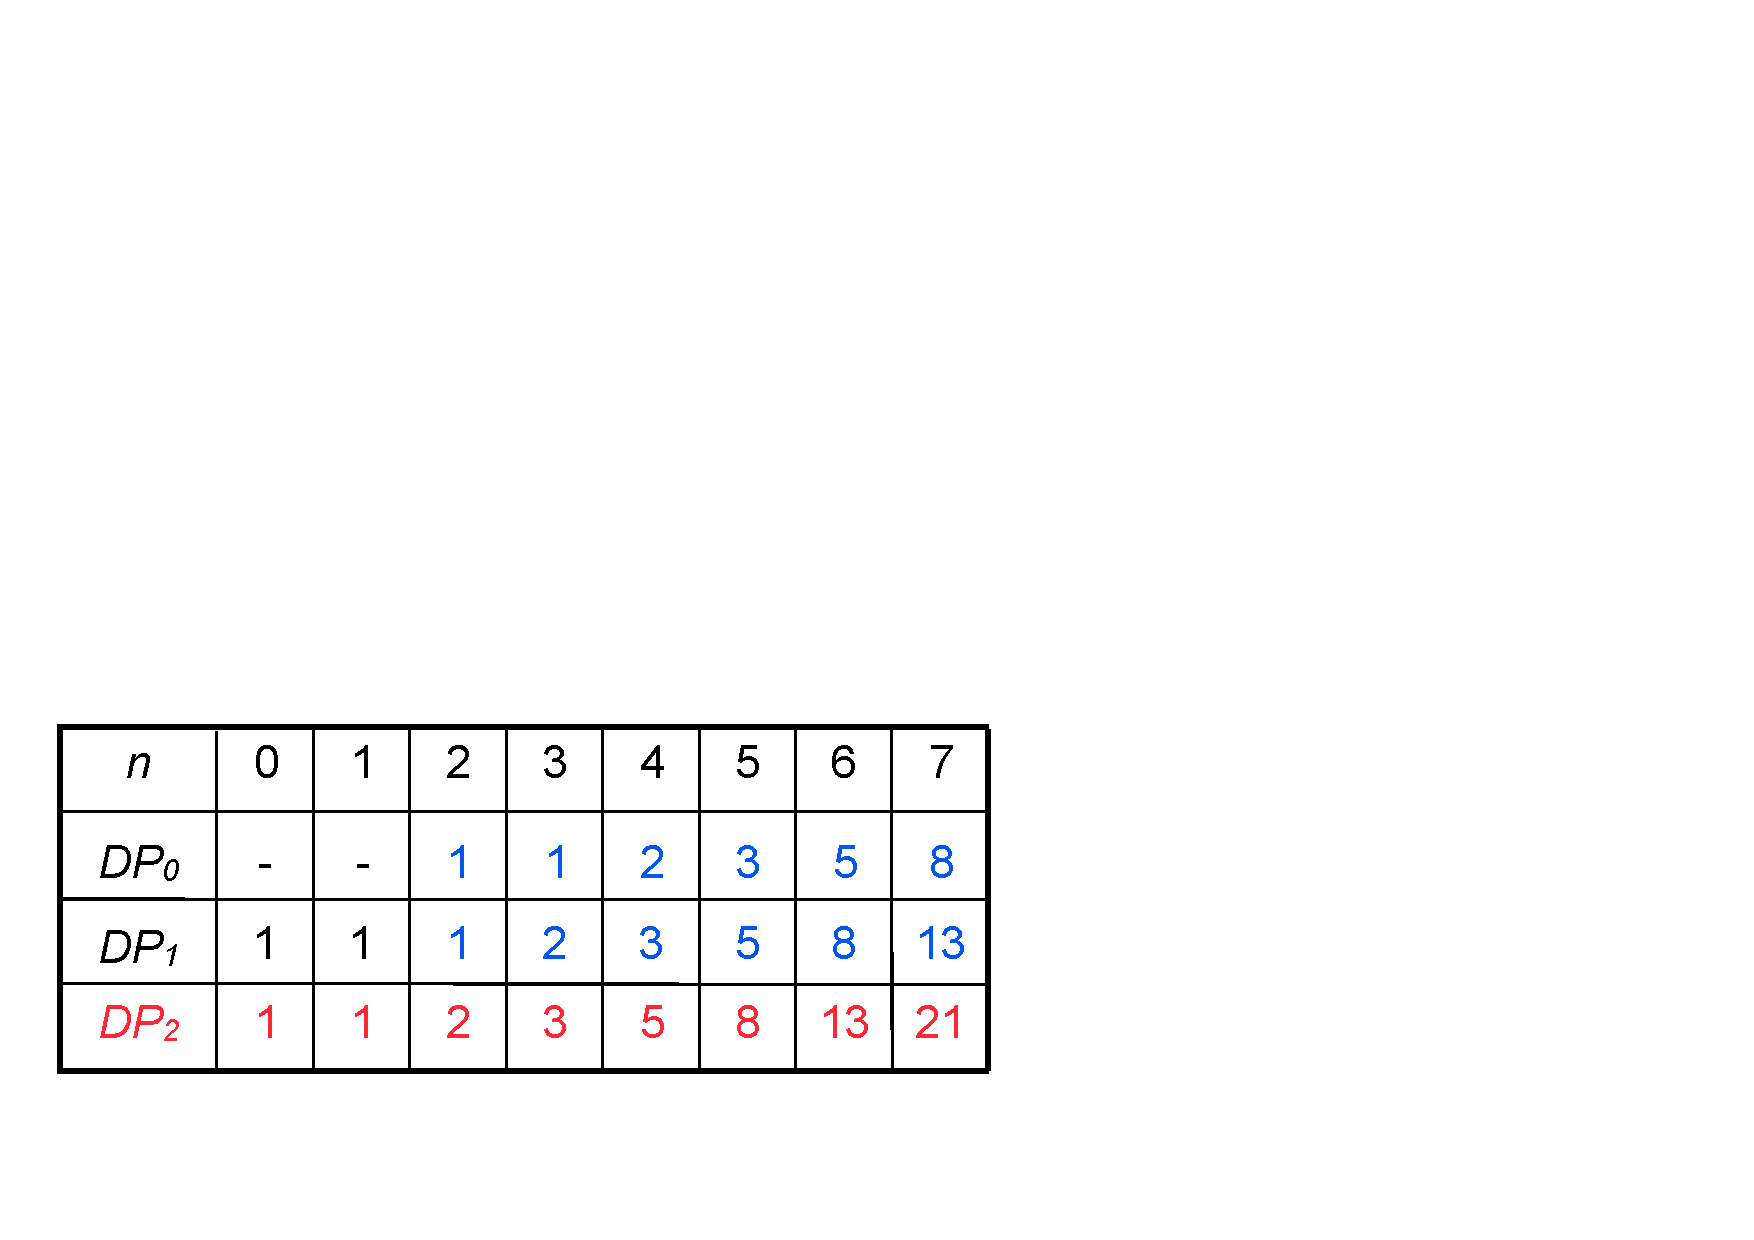
\includegraphics[width=\textwidth]{fib-table2.pdf}

\end{columns}

\begin{columns}[T]
\column{0.72\textwidth}
\BB{Qual è la complessità in \alert{spazio} di $\textsf{domino3}(n)$?}
\pause
\column{0.28\textwidth}
\bigskip
\alert{$S(n) = \Theta(1)$}
\end{columns}

\end{frame}



\begin{frame}[fragile]{Ripasso sulla complessità computazionale}

\vspace{-9pt}
\BB{Siete sicuri che i calcoli sulla complessità siano corretti?}

\pause
\bigskip
\BB{Osservate di nuovo la serie generata}

\begin{lstlisting}
1, 1, 2, 3, 5, 8, 13, 21, 34, 55, 89, 144, ...
\end{lstlisting}

\bigskip
\BB{Quanti bit sono necessari per memorizzare $F(n)$?}

\end{frame}


\begin{frame}{Modello costo uniforme vs modello costo logaritmico}

\vspace{-9pt}
\begin{myboxtitle}[Formula di Binet per i numeri di Fibonacci]
\vspace{6pt}
\begin{columns}[T]
\column{0.75\textwidth}
\[
DP(n-1) = F(n) = \frac{\phi^n}{\sqrt{5}} - \frac{(1-\phi)^n}{\sqrt{5}} 
\]
dove $\phi$ è la \alert{sezione aurea}:
\begin{align*}
\phi &={1+\sqrt 5 \over 2}=1{,}6180339887\dots  \\
\frac{1}{\phi} = \phi - 1 & ={2 \over 1+\sqrt 5 }=0{,}6180339887\dots 
\end{align*}
\column{0.20\textwidth}
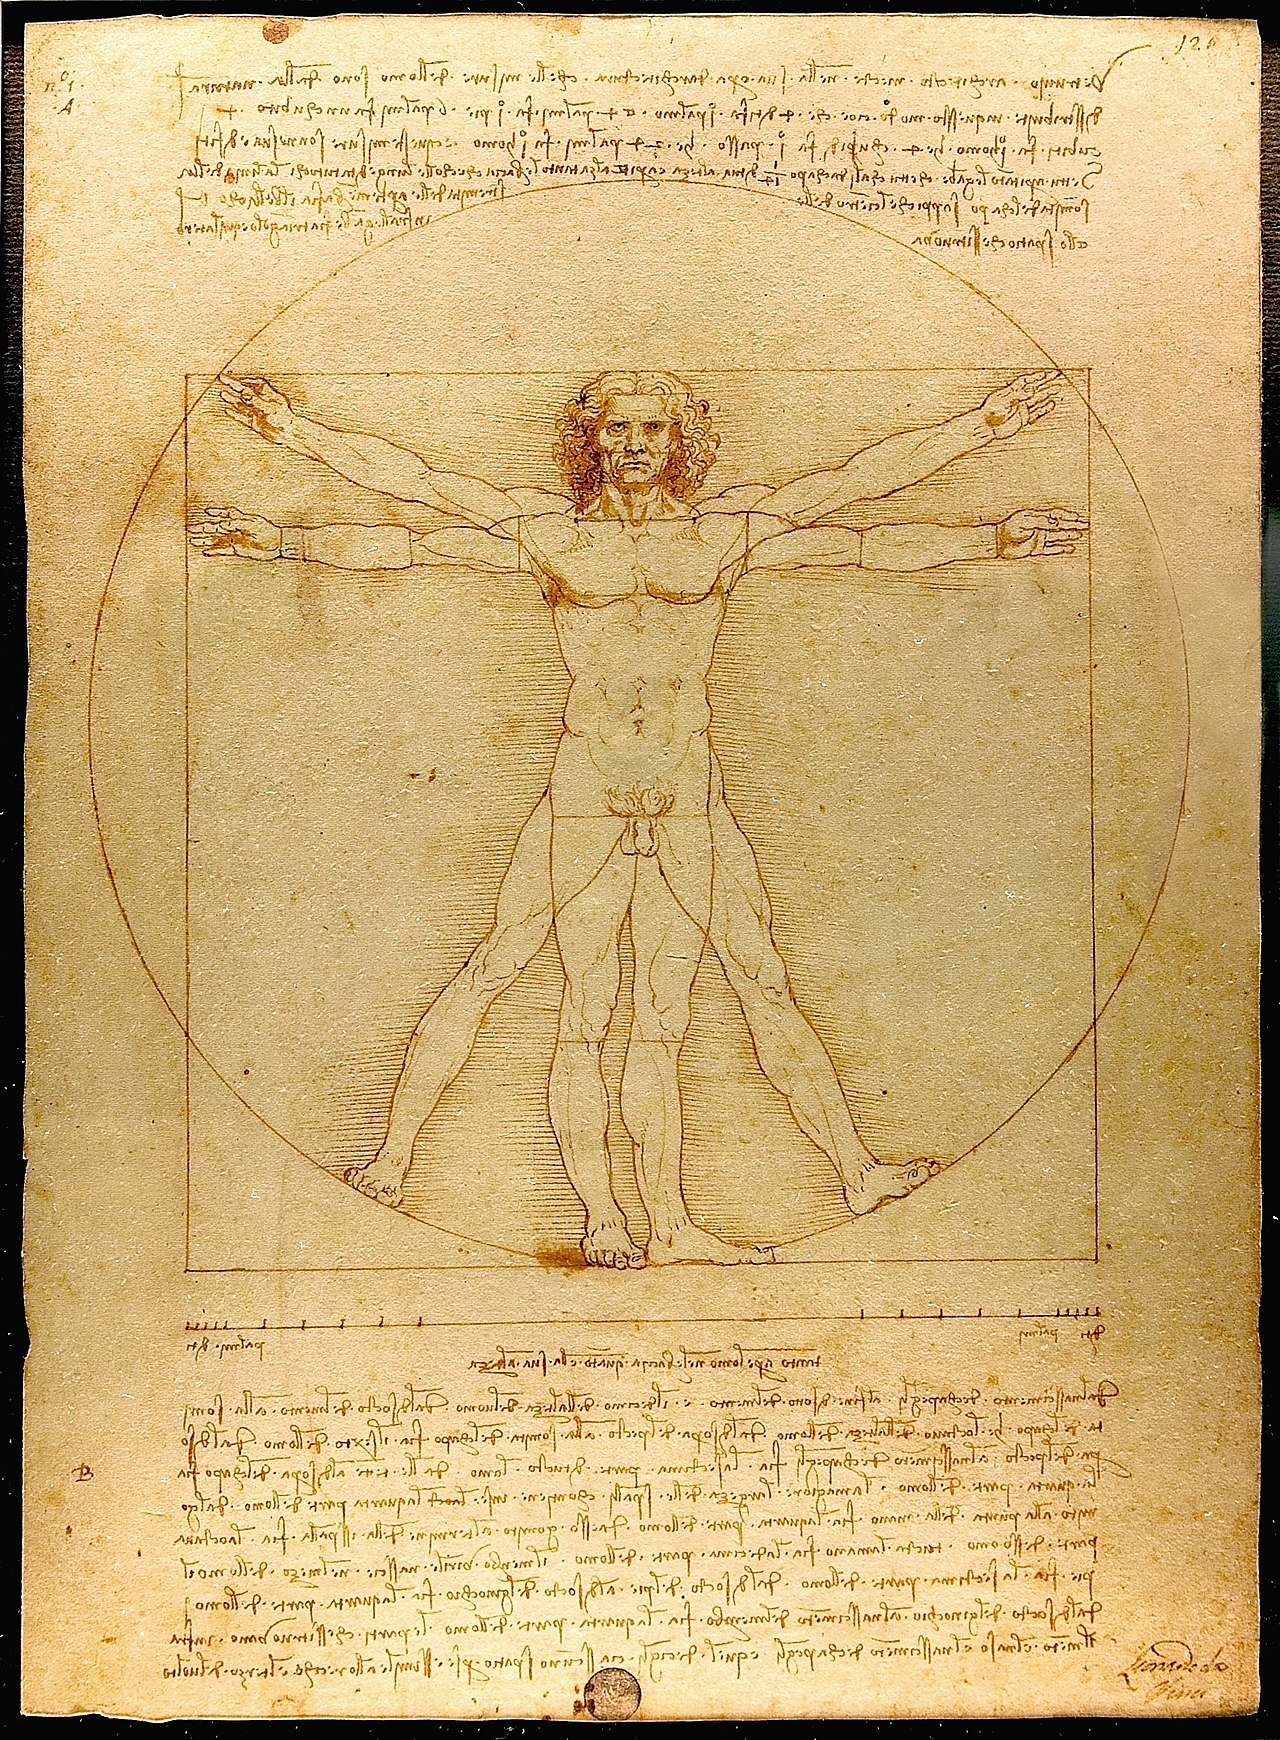
\includegraphics[width=\textwidth]{vitruviano.jpg}
\end{columns}
\end{myboxtitle}


\begin{columns}[T]
\column{0.75\textwidth}
\vspace{-6pt}
\BB{Quanti bit sono richiesti per memorizzare $F(n)$?}
\BB{Quanto costa sommare due numeri di Fibonacci consecutivi?}
\pause
\column{0.25\textwidth}

\bigskip
\alert{$\log F(n) = \Theta(n)$}
\end{columns}

\end{frame}

\begin{frame}{Modello costo uniforme vs modello costo logaritmico}
  
Sotto il modello di costo logaritmico, le tre versioni hanno la seguente
complessità:

\begin{center}
\begin{tabular}{|c|c|c|}
\hline
\textbf{Funzione} & \textbf{Complessità (Tempo)} & \textbf{Complessità (Spazio)} \\\hline
\textsf{domino1()} & $O(n2^n)$ & $O(n^2)$ \\\hline
\textsf{domino2()} & $O(n^2)$ & $O(n^2)$ \\\hline
\textsf{domino3()} & $O(n^2)$ & $O(n)$ \\\hline
\end{tabular}
\end{center}

\bigskip
Si può fare meglio di così utilizzando l'esponenziazione di matrici basata
su quadrati:

\bigskip
\url{https://brilliant.org/wiki/fast-fibonacci-transform/}


\end{frame}

%%%%%%%%%%%%%%%%%%%%%%%%%%%%%%%%%%%%%%%%%%%%%%%%%%%%%%%%%%%%%%%%%%%%%%%%%%%%%
\section{Hateville}
%%%%%%%%%%%%%%%%%%%%%%%%%%%%%%%%%%%%%%%%%%%%%%%%%%%%%%%%%%%%%%%%%%%%%%%%%%%%%

\begin{frame}{Hateville}

\BIL
\item Hateville è un villaggio particolare, composto da $n$ case, numerate da $1$ a 
$n$ lungo una singola strada. 

\item Ad Hateville ognuno odia i propri vicini della 
porta accanto, da entrambi i lati.
\item Quindi, il vicino $i$ odia i vicini $i-1$ e $i+1$ (se esistenti). 

\item Hateville vuole organizzare una sagra e vi 
ha affidato il compito di raccogliere i fondi. 

\item Ogni abitante $i$ ha intenzione
di  donare una quantità $D[i]$, ma non intende partecipare ad una raccolta 
fondi a cui partecipano uno o entrambi i propri vicini. 

\EIL

\end{frame}

\begin{frame}{Hateville}

Considerate i seguenti problemi:
\BIL
\item Scrivere un algoritmo che restituisca la quantità massima di
fondi che può essere raccolta
\item Scrivere un algoritmo che restituisca il sottoinsieme di indici 
$S \subseteq \{ 1, \ldots, n \}$ tale per cui la donazione totale
$T = \sum_{i \in S} D[i]$ è massimale
\EIL

\bigskip
\BB{Esempio}
\BIL
\item Vettore donazioni: \textsf{D = [4, 3, 6, 5]}
\item Raccolta fondi massima: 10
\item Insieme indici: $\{1, 3\}$
\EIL

\end{frame}

%-------------------------------------------------------------------------
\begin{frame}{Hateville}

\vspace{-9pt}
\BB{Come risolvereste il problema?}

\end{frame}

%-------------------------------------------------------------------------
\begin{frame}{Hateville}

Considerate i seguenti problemi:
\BIL
\item Scrivere un algoritmo che restituisca la quantità massima di
fondi che può essere raccolta
\item Scrivere un algoritmo che restituisca il sottoinsieme di indici 
$S \subseteq \{ 1, \ldots, n \}$ tale per cui la donazione totale
$T = \sum_{i \in S} D[i]$ è massimale
\EIL

\bigskip
\BB{Esempio}
\BIL
\item Vettore donazioni: \textsf{D = [10, 5, 5, 10]}
\item Raccolta fondi massima: 20
\item Insieme indici: $\{1, 4\}$
\EIL

\end{frame}


%-------------------------------------------------------------------------
\begin{frame}{Definizione ricorsiva}

\vspace{-9pt}
\begin{myboxtitle}[Definizione ricorrenza]
E' possibile definire una formula ricorsiva che ci permetta di calcolare
il sottoinsieme di case che, se selezionate, dà origine alla maggior quantità di donazioni?
\end{myboxtitle}

\bigskip
\BB{Ri-definiamo il problema}
\BIL
\item Sia $HV(i)$ uno dei possibili insiemi di indici da selezionare per ottenere una donazione ottimale dalle prime $i$ case di Hateville, numerate $1 \ldots n$ 
\item $HV(n)$ è la soluzione del problema originale
\EIL

\end{frame}

\begin{frame}{Passo ricorsivo}

\vspace{-9pt}
\BB{Considerate il vicino $i$-esimo}
\BI
\item Cosa succede se non accetto la sua donazione?
\EI
\[
HV(i) = \pause HV(i-1)
\]

\BI
\item Cosa succede se accetto la sua donazione?
\EI
\[
HV(i) = \pause \{ i \} \cup HV(i-2)  
\]

\BI
\item Come faccio a decidere se accettare o meno?
\EI
\[
HV(i) = \pause \mathit{highest}(HV(i-1), \{ i \} \cup HV(i-2)  )
\]

\end{frame}

\begin{frame}{Sottostruttura ottima -- Dimostrazione}

\BI
\item Sia $HV_p(i)$ il problema dato dalle prime $i$ case
\item Sia $HV_s(i)$ una soluzione ottima per il problema $HV_p(i)$
\item Sia $|HV_s(i)|$ il totale di donazioni di $HV_s(i)$
\EI

\begin{overprint}
\onslide<1|handout:1>
\BB{Caso 1: \alert{$i \not\in HV_s(i)$}}
\BIL
\item $HV_s(i)$ è una soluzione ottima anche per $HV_p(i-1)$
\item Se così non fosse, esisterebbe una soluzione $HV'_s(i-1)$ per il
problema $HV_p(i-1)$ tale che $|HV'_s(i-1)|>|HV_s(i)|$
\item Ma allora $HV'_s(i-1)$ sarebbe una soluzione per $HV_p(i)$ tale
che $|HV'_s(i-1)|>|HV_s(i)|$, assurdo
\EIL
\onslide<2|handout:2>
\BB{Caso 2: \alert{$i \in HV_s(i)$}}
\BIL
\item $i-1 \not\in HV_s(i)$, altrimenti non sarebbe una soluzione ammissibile
\item Quindi, $HV_s(i)-\{i\}$ è una soluzione ottima per $HV_p(i-2)$
\item Se così non fosse, esisterebbe una soluzione $HV'_s(i-2)$ per il
problema $HV_p(i-2)$ tale che $|HV'_s(i-2)|>|HV_s(i)-\{i\}|$
\item Ma allora $HV'_s(i-2) \cup \{i \}$ sarebbe una soluzione per $HV_p(i)$
tale che $|HV'_s(i-2) \cup \{i\}|>|HV_s(i)|$, assurdo
\EIL
\end{overprint}


\end{frame}



\begin{frame}{Completare la ricorsione}

\vspace{-9pt}
\BB{Quali sono i casi base?}
\pause
\BIL
\item $HV(0) = \emptyset$
\item $HV(1) = \{ 1 \}$
\EIL

\BB{Tutto insieme!}

\[
HV(i) = \begin{cases}
  \emptyset & i=0 \\
  \{ 1 \} & i=1 \\
  \mathit{highest}(HV(i-1), HV(i-2) \cup \{ i \}) & i \geq 2
  \end{cases}
\]

\end{frame}

\begin{frame}{Algoritmo ricorsivo}

\vspace{-9pt}
\begin{myboxtitle}[Domanda]
Vale la pena scrivere un algoritmo ricorsivo, basato su divide-et-impera,
per risolvere il problema di Hateville?
\end{myboxtitle}

\bigskip
\begin{overprint}
\onslide<1|handout:0>
\[
HV(i) = \begin{cases}
  \emptyset & i=0 \\
  \{ 1 \} & i=1 \\
  \mathit{highest}(HV(i-1), HV(i-2) \cup \{ i \}) & i \geq 2
  \end{cases}
\]
\onslide<2|handout:1>
\IG{1.0}{fibonacci-tree.pdf}
\end{overprint}

\end{frame}

\begin{frame}{Memorizzare una tabella}

\vspace{-9pt}
\begin{myboxtitle}[Esempi]
\small
%|P{0.50cm}|P{0.50cm}|P{0.5cm}|P{0.5cm}|P{1.1cm}|P{1.1cm}|P{1.1cm}|P{1.1cm}|P{1.1cm}|P{1.3cm}|
\medskip
\begin{tabular}{|c|c|c|c|c|c|c|c|c|}
\hline
$i$ & 0 & 1 & 2 & 3 & 4 & 5 & 6 & 7 \\\hline
$D$ &   & 10 & 5 & 5 & 8 & 4 & 7 & 12 \\\hline
$HV$ & $\emptyset$ & $\{ 1 \}$ & $\{ 1 \}$ & $\{ 1,3 \}$ & $\{ 1,4 \}$ & $\{ 1,3,5 \}$ & $ \{ 1,4,6 \}$ & $\{ 1,3,5,7 \}$ \\\hline
\end{tabular}

\medskip
%|P{0.50cm}|P{0.50cm}|P{0.5cm}|P{0.5cm}|P{1.1cm}|P{1.1cm}|P{1.1cm}|P{1.1cm}|P{1.1cm}|P{1.3cm}|
\begin{tabular}{|c|c|c|c|c|c|c|c|c|}
\hline
$i$ & 0 & 1 & 2 & 3 & 4 & 5 & 6 & 7 \\\hline
$D$ &   & 10 & 1 & 1 & 10 & 1 & 1 & 10 \\\hline
$HV$ & $\emptyset$ & $\{ 1 \}$ & $\{ 1 \}$ & $\{ 1,3 \}$ & $\{ 1,4 \}$ & $\{ 1, 4 \}$ & $ \{ 1,4,6 \}$ & $\{ 1,4,7 \}$ \\\hline
\end{tabular}
\end{myboxtitle}

\begin{myboxtitle}[Problemi]
\BIL
\item Dobbiamo definire la funzione $\mathit{highest}()$
\item \alert{Memorizzare gli insiemi nella tabella è costoso}
\EIL
\end{myboxtitle}

\end{frame}

\begin{frame}{Tabella DP}

\vspace{-9pt}
\begin{myboxtitle}[Valore della soluzione ottima]
\BIL
\item Sia $DP(i)$ il \alert{valore} della massima quantità di donazioni che possiamo
ottenere dalle prime $i$ case di Hateville. 
\item $DP(n)$ è il valore della soluzione ottima
\EIL
\end{myboxtitle}

\begin{overprint}
\onslide<1|handout:0>
\[
  DP(i) =
  \begin{cases}
   \makebox[6cm][l]{?} & i = 0 \\
   \makebox[6cm][l]{?} & i = 1 \\
   \makebox[6cm][l]{?} & i \geq 2 
   \end{cases}
\]
\onslide<2|handout:0>
\[
  DP(i) =
  \begin{cases}
   0 & i = 0 \\
  \makebox[6cm][l]{?} & i = 1 \\
  \makebox[6cm][l]{?} & i \geq 2 
   \end{cases}
\]
\onslide<3|handout:0>
\[
  DP(i) =
  \begin{cases}
   0 & i = 0 \\
   D[1] & i = 1 \\
  \makebox[6cm][l]{?} & i \geq 2 
   \end{cases}
\]
\onslide<4|handout:1>
\[
  DP(i) =
  \begin{cases}
   0 & i = 0 \\
   D[1] & i = 1 \\
   \max(DP(i-1), DP(i-2) + D[i]) & i \geq 2 
   \end{cases}
\]
\end{overprint}

\end{frame}

\begin{frame}{Hateville: Algoritmo iterativo}

\vspace{-9pt}
\BB{Algoritmo iterativo che risolve il problema Hateville}

\pause
\begin{Procedure}
\caption[A]{\textsf{hateville}($\INTEGER[\,]\ D$, \INTEGER $n$)}
$\INTEGER[\,]\ DP = \NEW\ \INTEGER[0 \ldots n]$\;
$DP[0] = 0$\;
$DP[1] = D[1]$\;
\For{$i = 2$ \TO\ $n$}{
  $DP[i] = \MAX(DP[i-1], DP[i-2]+D[i])$\;
}
\Return $DP[n]$\;
\end{Procedure}

\end{frame}

\begin{frame}[fragile]{Sulla risoluzione con "veri" linguaggi di programmazione}

\begin{lstlisting}[language=java]
public int hateville(int[] D, int n) {
  int[] DP = new int[n+1];
  DP[0] = 0;
  DP[1] = <@\color{blue}{D[0]}@>;
  for (int i=2; i <= n; i++) {
    DP[i] = max(DP[i-1],DP[i-2]+<@\color{blue}{D[i-1]}@>);
  }
  return DP[n];
}
\end{lstlisting}

\begin{lstlisting}[language=python]
def hateville(D):
  DP = [ 0, <@\color{blue}{D[0]}@> ]
  for i in range(<@\color{blue}{1,len(D)}@>):
    DP.append( max(DP[-1], DP[-2] + D[i]) )
  return DP[-1]
\end{lstlisting}


\end{frame}



\begin{frame}{Memorizzare una tabella}

\vspace{-9pt}
\begin{myboxtitle}[Esempi]
\begin{center}
%|P{0.50cm}|P{0.50cm}|P{0.5cm}|P{0.5cm}|P{1.1cm}|P{1.1cm}|P{1.1cm}|P{1.1cm}|P{1.1cm}|P{1.3cm}|
\medskip
\begin{tabular}{|c|c|c|c|c|c|c|c|c|}
\hline
$i$ & 0 & 1 & 2 & 3 & 4 & 5 & 6 & 7 \\\hline
$D$ &   & 10 & 5 & 5 & 8 & 4 & 7 & 12 \\\hline
$DP$ & 0 & 10 & 10 & 15 & 18 & 19 & 25 & 31 \\\hline
\end{tabular}

\medskip
%|P{0.50cm}|P{0.50cm}|P{0.5cm}|P{0.5cm}|P{1.1cm}|P{1.1cm}|P{1.1cm}|P{1.1cm}|P{1.1cm}|P{1.3cm}|
\begin{tabular}{|c|c|c|c|c|c|c|c|c|}
\hline
$i$ & 0 & 1 & 2 & 3 & 4 & 5 & 6 & 7 \\\hline
$D$ &   & 10 & 1 & 1 & 10 & 1 & 1 & 10 \\\hline
$DP$ & 0 & 10 & 10 & 11 & 20 & 20 & 21 & 30 \\\hline
\end{tabular}
\end{center}
\end{myboxtitle}

\begin{myboxtitle}[Problema]
Abbiamo il valore della soluzione massimale, ma non abbiamo
la soluzione!
\end{myboxtitle}

\end{frame}

\begin{frame}[fragile]{Ricostruire la soluzione originale}

\vspace{-9pt}
\BB{Approccio}
\BIL
\item Si guarda l'elemento $DP[i]$. Da cosa deriva il suo valore?
  \BI 
  \item Se $DP[i] = DP[i-1]$, la casa $i$ non è stata selezionata
  \item Se $DP[i] = DP[i-2]+D[i]$, la casa $i$ è stata selezionata
  \item Se entrambe le equazioni sono vere, una vale l'altra!
  \EI
\item Utilizziamo questa informazione per ricostruire la soluzione in modo
  ricorsivo:
  \BI
  \item Per ricostruire la soluzione fino ad $i$,
  ricostriamo la soluzione fino ad $i-2$ e aggiungiamo $i$
  \item Oppure, ricostriuamo la soluzione fino ad $i-1$ senza aggiungere nulla
  \EI
\EIL

\end{frame}

\begin{frame}[fragile]{Ricostruire la soluzione originale}

\vspace{-12pt}
\TwoColsCustom{0.57}{0.42}{
\begin{Procedure}
\caption[A]{\Set\ \textsf{solution}($\INTEGER[\,]\ DP$, $\INTEGER[\,]\ D$, \INTEGER $i$)}
\uIf{$i \Eq 0$}{
  \Return $\emptyset$
}
\uElseIf{$i \Eq 1$}{
  \Return $\{ 1 \}$
}
\uElseIf{$DP[i]  \Eq  DP[i-1]$}{
  \Return $\textsf{solution}(DP, D, i-1)$\;
}
\Else{
  $\Set\ \mathit{sol} = \textsf{solution}(DP, D, i-2)$\;
  $\mathit{sol}.\textsf{insert}(i)$\;
  \Return $\mathit{sol}$\;
}
\end{Procedure}
}
{
\begin{Procedure}
\caption[A]{\textsf{hateville}($\INTEGER[\,]\ D$, \INTEGER $n$)}
[...]\;
\Return $\textsf{solution}(DP, D, n)$\;
\end{Procedure}
}
\end{frame}

\begin{frame}{Complessità computazionale}

\vspace{-9pt}
\onslide<1-|handout:1->
\BB{Qual è la complessità computazionale di \textsf{solution()}?}
\onslide<2-|handout:1->
\medskip  
$T(n) = \Theta(n)$

\bigskip
\onslide<1-|handout:1->
\BB{Qual è la complessità computazionale e spaziale di \textsf{hateville()}?}
\onslide<3-|handout:1->
\medskip  
$T(n) = \Theta(n) \qquad S(n) = \Theta(n)$

\bigskip
\onslide<1-|handout:1->
\BB{E' possibile migliorare la complessità spaziale di \textsf{hateville()}?}
\onslide<4-|handout:1->
\medskip
No, se vogliamo ricostruire la soluzione.

\end{frame}

%%%%%%%%%%%%%%%%%%%%%%%%%%%%%%%%%%%%%%%%%%%%%%%%%%%%%%%%%%%%%%%%%%%%%%%%%%%%%
\section{Zaino}
%%%%%%%%%%%%%%%%%%%%%%%%%%%%%%%%%%%%%%%%%%%%%%%%%%%%%%%%%%%%%%%%%%%%%%%%%%%%%

\begin{frame}{Zaino (Knapsack)}

\vspace{-9pt}
\begin{myboxtitle}[Descrizione del problema]
Dato un insieme di oggetti, ognuno caratterizzato da un \alert{peso} e un \alert{profitto},
e uno "zaino" con un limite di capacità, individuare un sottoinsieme di oggetti 
\BIL
\item il cui peso sia inferiore alla capacità dello zaino;\
\item il valore totale degli oggetti sia massimale, i.e.
più alto o uguale al valore di qualunque altro sottoinsieme di oggetti 
\EIL
\end{myboxtitle}

\begin{center}
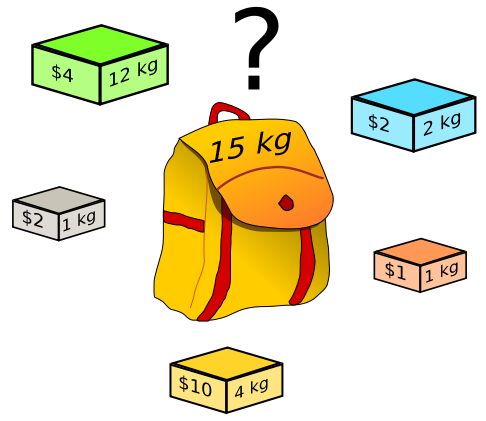
\includegraphics[width=0.3\textwidth]{knapsack.png}
\end{center}

\footnotesize
\url{https://en.wikipedia.org/wiki/Knapsack_problem\#/media/File:Knapsack.svg}


\end{frame}

\begin{frame}{Zaino}

\vspace{-9pt}
\begin{myboxtitle}[Input]
\BIL
\item Vettore $w$, dove \alert{$w[i]$} è il \alert{peso} (\alert{weight}) dell'oggetto $i$-esimo
\item Vettore $p$, dove \alert{$p[i]$} è il \alert{profitto} (\alert{profit}) dell'oggetto $i$-esimo
\item La \alert{capacità} $C$ dello zaino
\EIL
\end{myboxtitle}

\begin{myboxtitle}[Output]
Un insieme $S \subseteq \{1, \ldots, n\}$ tale che:

\medskip
\begin{tabular}{P{5cm}P{5cm}}
Il \alert{volume totale} deve essere minore o uguale alla capacità &

$w(S) = \sum_{i \in S} w[i] \leq C$
\\
~\\
Il \alert{profitto totale} deve essere massimizzato &
$
p(S) = \sum_{i \in S} p[i]
$
\\
\end{tabular}
\end{myboxtitle}

\end{frame}

\begin{frame}{Esempi}

\vspace{-9pt}
\BB{Quali sono gli oggetti migliori per questo esempio?}

\begin{columns}[T]
\column{0.40\textwidth} 
\begin{tabular}{|r|c|c|c|}
\hline
\textbf{Item id} & \textbf{1} & \textbf{2} & \textbf{3} \\\hline
\textbf{Weight} & 10 & 4 & 8 \\\hline
\textbf{Profit} & 20 & 6 & 12 \\\hline 
\end{tabular} 
\column{0.15\textwidth}
\[C=12\]
\pause
\column{0.35\textwidth}
\[S = \{1 \}\]
\end{columns}

\smallskip
\BB{Progettare un algoritmo che risolve il problema dello zaino}

\pause
\smallskip
\BB{Il vostro algoritmo funziona per questo esempio?}

\begin{columns}[T]
\column{0.40\textwidth}
\begin{tabular}{|r|c|c|c|}
\hline
\textbf{Item id} & \textbf{1} & \textbf{2} & \textbf{3} \\\hline
\textbf{Weight} & 10 & 4 & 8 \\\hline
\textbf{Profit} & 20 & 7 & 15 \\\hline 
\end{tabular}
\column{0.15\textwidth}
\[C=12\]
\pause
\column{0.35\textwidth}
\[S = \{ 2,3 \}\]
\end{columns}
\end{frame}

\begin{frame}{Definizione matematica del valore della soluzione}

\vspace{-9pt}
\begin{myboxtitle}[Valore della soluzione]
Dato uno zaino di capacità $C$ e $n$ oggetti caratterizzati
da peso $w$ e profitto $p$, definiamo $DP(i,c)$ come il
massimo profitto che può essere ottenuto dai primi $i \leq n$
oggetti contenuti in uno zaino di capacità $c \leq C$.
\end{myboxtitle}

\begin{myboxtitle}[Problema originale]
Il massimo profitto ottenibile dal problema originale è rappresentato da $DP(n, C)$.
\end{myboxtitle}

\end{frame}


\begin{frame}{Parte ricorsiva}

\vspace{-9pt}
\BB{Considerate l'ultimo oggetto}

\bigskip
\begingroup
\renewcommand*{\arraystretch}{1.2}
\begin{tabular}{P{2.8cm}P{3.9cm}P{4.0cm}}
Cosa succede se non lo prendete? & $DP(i,c) = \pause\newline DP(i-1,c)$ & La capacità non cambia, non c'è profitto \\
~\\
Cosa succede se lo prendete? & $DP(i,c) = \pause DP(i-1,c-w[i]) + p[i]$ & Sottraete il peso dalla capacità e aggiungete il profitto relativo \\
\end{tabular}
\endgroup

\BB{Come scegliere la soluzione migliore?}

\[
DP(i,c) = \pause \max( DP(i-1,c-w[i]) + p[i], DP(i-1,c) )
\]

\end{frame}


\begin{frame}{Casi base}

\vspace{-9pt}
\BB{Quali sono i casi base?}

\pause
\BIL
\item Qual è il profitto massimo se non avete più oggetti?
\item Qual è il profitto massimo se non avete più capacità?
\item Cosa succede se la capacità è negativa?
\EIL

\pause
\[
DP(i,c) = \begin{cases}
  0 & i=0\ \OR\ c=0 \\
  -\infty & c < 0
\end{cases}
\]

\end{frame}

\begin{frame}{Formula completa}

\begingroup
\small
\[
DP(i,c) = \begin{cases}
  0 & i=0\ \OR\ c=0 \\
  -\infty & c < 0 \\
  \max( DP(i-1,c-w[i]) + p[i], DP(i-1,c) ) & \textrm{otherwise}
\end{cases}
\]
\endgroup

Come trasformare questa formula in un algoritmo?

\end{frame}

%-------------------------------------------------------------------------
\begin{frame}{Zaino}

\vspace{-9pt}
\begin{Procedure}
\caption[A]{\INTEGER\ \textsf{knapsack}($\INTEGER[\,]\ w$, $\INTEGER[\,]\ p$, \INTEGER\ $n$, \INTEGER\ $C$)}

$DP = \NEW\ \INTEGER[0 \ldots n][0 \ldots C]$\;
\For{$i = 0$ \TO\ $n$}{
  $DP[i][0] = 0$\;
}
\For{$c = 0$ \TO\ $C$}{
  $DP[0][c] = 0$\;
}
\For{$i = 1$ \TO\ $n$}{
  \For{$c = 1$ \TO\ $C$}{
    \eIf{$w[i] \leq c$}{
      \vspace{-12pt}
      $DP[i][c] = \MAX(\overbrace{DP[i-1][c-w[i]]+p[i]}^{\textrm{Taken}},\overbrace{DP[i-1][c]}^{\textrm{Not taken}})$\;
    }{
      \vspace{-12pt}
      $DP[i][c] = \overbrace{DP[i-1][c]}^{\textrm{Not taken}}$\;
    }
  }
}
\Return{$DP[n][C]$}\;
\end{Procedure}

\end{frame}


\begin{frame}[fragile]{Esempio}

\begin{lstlisting}
w = [ 4, 2, 3, 4]
p = [10, 7, 8, 6]
C = 9  
\end{lstlisting}

\bigskip
\begin{tabular}{|c|c|c|c|c|c|c|c|c|c|c|}
\hline
& \multicolumn{10}{c|}{$c$} \\\hline
$i$ & \textbf{0} & \textbf{1} & \textbf{2} & \textbf{3} & \textbf{4} & \textbf{5} & \textbf{6} & \textbf{7} & \textbf{8} & \textbf{9}  \\\hline
\textbf{0} & 0 &  0 &  0 &  0 &  0 &  0 &  0 &  0 &  0 &  0 \\\hline
\textbf{1} & 0 &  0 &  0 &  0 & 10 & 10 & 10 & 10 & 10 & 10 \\\hline
\textbf{2} & 0 &  0 &  7 &  7 & 10 & 10 & 17 & 17 & 17 & 17 \\\hline
\textbf{3} & 0 &  0 &  7 &  8 & 10 & 15 & 17 & 18 & 18 & 25 \\\hline
\textbf{4} & 0 &  0 &  7 &  8 & 10 & 15 & 17 & 18 & 18 & 25 \\\hline  
\end{tabular}  

\end{frame}

\begin{frame}[fragile]{Complessità computazionale}

\BB{Qual è la complessità della funzione \textsf{knapsack()}?}

\begin{overprint}
\onslide<1|handout:0>
\begingroup
\footnotesize
\begin{Procedure}
\caption[A]{\INTEGER\ \textsf{knapsack}($\INTEGER[\,]\ w$, $\INTEGER[\,]\ p$, \INTEGER\ $n$, \INTEGER\ $C$)}

$DP = \NEW\ \INTEGER[0 \ldots n][0 \ldots C]$\;
\For{$i = 0$ \TO\ $n$}{
  $DP[i][0] = 0$\;
}
\For{$c = 0$ \TO\ $C$}{
  $DP[0][c] = 0$\;
}
\For{$i = 1$ \TO\ $n$}{
  \For{$c = 1$ \TO\ $C$}{
    \eIf{$w[i] \leq c$}{
      $DP[i][c] = \MAX(DP[i-1][c-w[i]]+p[i],DP[i-1][c])$\;
    }{
      $DP[i][c] = DP[i-1][c]$\;
    }
  }
}
\Return{$DP[n][C]$}\;
\end{Procedure}
\endgroup
\onslide<2|handout:0>
\[ 
  T(n) = O(nC)
\]

\BB{E' un algoritmo polinomiale?}

\onslide<3|handout:1>
\[ 
  T(n) = O(nC)
\]

\BB{E' un algoritmo polinomiale?}

\medskip
No, è un algoritmo \alert{pseudo-polinomiale}, perchè sono necessari \alert{$k = \log C$} bit
per rappresentare $C$ e quindi la complessità è:

\[
  \alert{T(n) = O(n 2^k) }
\]
\end{overprint}

\end{frame}


\begin{frame}{Zaino ricorsivo}

\vspace{-12pt}
\begin{Procedure}
\caption[A]{\textsf{knapsack}($\INTEGER[\,]\ w$, $\INTEGER[\,]\ p$, \INTEGER\ $n$, \INTEGER\ $C$)}
\Return $\textsf{knapsackRec}(w, p, n, C)$
\end{Procedure}

\vspace{-15pt}
\begin{Procedure}
\caption[A]{\INTEGER\ \textsf{knapsackRec}($\INTARRAY\ w$,\ $\INTARRAY\ p$,\  \INTEGER\ $i$,\ \INTEGER\ $c$)}

\uIf{$c < 0$}{\Return $-\infty$\;}
\uElseIf{$i  \Eq  0$ \OR\ $c  \Eq  0$}{\Return 0\;}
\Else{
$\INTEGER\ \mathit{nottaken} = \textsf{knapsackRec}(w,p, i-1, c)$\;
$\INTEGER\ \mathit{taken} = \textsf{knapsackRec}(w,p,i-1,c-w[i])+p[i]$\;
\Return $\MAX(nottaken, taken)$\;
}
\end{Procedure}

\vspace{-6pt}
\BB{Qual è la complessità della funzione \textsf{knapsack()} ricorsiva?}

\end{frame}


\begin{frame}[fragile]{Complessità computazionale}

\vspace{-9pt}
\BB{Qual è la complessità della funzione \textsf{knapsack()} ricorsiva?}

\begin{align*}
T(n) &= \begin{cases}
  1 & n \leq 1 \\
  2T(n-1)+1 & n>1
\end{cases}\\
  T(n) &= O(2^n)
\end{align*}

\BB{E' un algoritmo polinomiale?}

\medskip
Ovviamente no!

\bigskip
\BB{Possiamo fare meglio di così?}

\medskip
No, secondo l'\alert{opinione} di quasi tutti gli informatici del mondo.

\end{frame}


\begin{frame}[fragile]{Memoization}

\vspace{-9pt}
\BB{Osservazione}
Non tutti gli elementi della matrice sono necessari alla risoluzione del
nostro problema.

\begin{lstlisting}
w = [ 4, 2, 3, 4]
p = [10, 7, 8, 6]       C = 9  
\end{lstlisting}

\bigskip
\begin{tabular}{|c|c|c|c|c|c|c|c|c|c|c|}
\hline
& \multicolumn{10}{c|}{$c$} \\\hline
$i$ & \textbf{0} & \textbf{1} & \textbf{2} & \textbf{3} & \textbf{4} & \textbf{5} & \textbf{6} & \textbf{7} & \textbf{8} & \textbf{9}  \\\hline
\bf{0} & \alert{\bf 0} &  \alert{\bf 0} &  \alert{\bf 0} &  \alert{\bf 0} &  \alert{\bf 0} &  \alert{\bf 0} &  \alert{\bf 0} &  \alert{\bf 0} &  0 &  \alert{\bf 0} \\\hline
\bf{1} & \alert{\bf 0} &  0 &  \alert{\bf 0} & \alert{\bf 0} & \alert{\bf 10} & \alert{\bf 10} & \alert{\bf 10} & \alert{\bf 10} & 10 & \alert{\bf 10} \\\hline
\bf{2} & 0 &  0 &  \alert{\bf 7} &  7 & 10 & \alert{\bf 10} & \alert{\bf 17} & 17 & 17 & \alert{\bf 17} \\\hline
\bf{3} & 0 &  0 &  7 &  8 & 10 & \alert{\bf 15} & 17 & 18 & 18 & \alert{\bf 25} \\\hline
\bf{4} & 0 &  0 &  7 &  8 & 10 & 15 & 17 & 18 & 18 & \alert{\bf 25} \\\hline  
\end{tabular}  
  
\end{frame}


%-------------------------------------------------------------------------
\begin{frame}{Memoization}

\vspace{-9pt}
\begin{myboxtitle}[Memoization (annotazione)]
Tecnica che fonde l'approccio di memorizzazione della programmazione dinamica con l'approccio top-down di divide-et-impera
\end{myboxtitle}

\BIL
\item Si crea una tabella $DP$, inizializzata con un \alert{valore speciale} ad 
indicare che un certo sottoproblema non è ancora stato risolto
\item Ogni volta che si deve risolvere un sottoproblema, si controlla nella tabella se è già stato risolto precedentemente
\BI
\item SI:  si usa il risultato della tabella
\item NO:  si calcola il risultato e lo si memorizza
\EI
\item In tal modo, ogni sottoproblema viene calcolato una sola volta e memorizzato come nella versione bottom-up
\EIL

\end{frame}

\begin{frame}{Zaino con memoization}

\vspace{-9pt}
\begin{Procedure}
\caption[A]{\textsf{knapsack}($\INTEGER[\,]\ w$, $\INTEGER[\,]\ p$, \INTEGER\ $n$, \INTEGER\ $C$)}
\alert{$DP = \NEW\ \INTEGER[1 \ldots n][1 \ldots C]$\;
\For{$i = 1$ \TO $n$}{
  \For{$c = 1$ \TO $C$}{
    $DP[i][c] = -1$\;
  }
}}
\Return $\textsf{knapsackRec}(w, p, n, C, \alert{DP})$
\end{Procedure}

\BIL
\item La tabella viene inizializzata esternamente, nella funzione wrapper
\item Il valore -1 è scelto per indicare una cella non ancora calcolata
\EIL

\end{frame}

\begin{frame}{Zaino con memoization}

\vspace{-9pt}
\begin{Procedure}
\caption[A]{\INTEGER\ \textsf{knapsackRec}($\INTARRAY\ w,\ \INTARRAY\ p,\  \INTEGER\ i,\ \INTEGER\ c,\ \alert{\INTARRAY[\,]\ DP}$)}

\uIf{$c < 0$}{
  \Return $-\infty$\;
}
\uElseIf{$i \Eq 0$ \OR\ $c \Eq 0$}{
  \Return 0\;
}
\Else{
  \If{\alert{$DP[i][c] < 0$}}{
    $\INTEGER\ \mathit{nottaken} = \textsf{knapsackRec}(w,p, i-1, c, \alert{DP})$\;
    $\INTEGER\ \mathit{taken} = \textsf{knapsackRec}(w,p,i-1,c-w[i], \alert{DP})+p[i]$\;
    $\alert{DP[i][c]} = \MAX(nottaken, taken)$\;
  }
  \Return $\alert{DP[i][c]}$\;
}
\end{Procedure}

\end{frame}



%-------------------------------------------------------------------------
\begin{frame}[fragile,shrink=5]{Zaino con memoization}

\vspace{-9pt}
\begin{lstlisting}[language=python,tabsize=2]
def knapsackRec(w, p, i, c, DP):
	if c < 0:
		return -math.inf
	elif i == 0 or c == 0:
		return 0
	else:
		if DP[i][c] < 0:
			nottaken = knapsackRec(w, p, i-1, c, DP)
			taken = knapsackRec(w, p, i-1, c-w[<@\color{blue}{i-1}@>], DP) + p[<@\color{blue}{i-1}@>]
			DP[i][c] = max(nottaken, taken)
		return DP[i][c]

def knapsack(w,p,C):
	n = len(w)
	DP = [[-1]*(C+1) for i in range(n+1)]
	return knapsackRec(w,p,n,C,DP)
\end{lstlisting}

\end{frame}

\begin{frame}[fragile]{Esempio}

\begin{lstlisting}
w = [ 4, 2, 3, 4]
p = [10, 7, 8, 6]
C = 9  
\end{lstlisting}

\bigskip
\begin{tabular}{|c|c|c|c|c|c|c|c|c|c|c|}
\hline
& \multicolumn{10}{c|}{$c$} \\\hline
$i$ & \textbf{0} & \textbf{1} & \textbf{2} & \textbf{3} & \textbf{4} & \textbf{5} & \textbf{6} & \textbf{7} & \textbf{8} & \textbf{9}  \\\hline
\bf{0} & 0 &  0 &  0 &  0 &  0 &  0 &  0 &  0 &  0 &  0 \\\hline
\bf{1} & 0 &  -1 &  \alert{\bf 0} &  \alert{\bf 0} & \alert{\bf 10} & \alert{\bf 10} & \alert{\bf 10} & \alert{\bf 10} & -1 & \alert{\bf 10} \\\hline
\bf{2} & 0 &  -1 &  \alert{\bf 7} & -1 & -1 & \alert{\bf 10} & \alert{\bf 17} & -1 & -1 & \alert{\bf 17} \\\hline
\bf{3} & 0 &  -1 &  -1 &  -1 & -1 & \alert{\bf 15} & -1 & -1 & -1 & \alert{\bf 25} \\\hline
\bf{4} & 0 &  -1 &  -1 &  -1 & -1 & -1 & -1 & -1 & -1 & \alert{\bf 25} \\\hline  
\end{tabular}  
  
\end{frame}

\begin{frame}{Dizionario vs tabella}

\vspace{-9pt}
\BB{Inizializzazione tabella}
  \BIL
  \item Il costo di inizializzazione è pari a $O(nC)$
  \item Applicata in questo modo, non c'è alcun vantaggio nell'utilizzare
  la tecnica di memoization
  \item Permette tuttavia di tradurre in fretta le espressioni ricorsive
  \EIL

\pause
\BB{Utilizzo di un dizionario (hash table)}
  \BIL
  \item Invece di utilizzare una tabella, si utilizza un dizionario
  \item Non è necessario fare inizializzazione
  \item Il costo di esecuzione è pari a $O(\min(2^n,nC))$
  \EIL

\end{frame}

\begin{frame}[fragile,shrink=5]{Zaino con dizionario (Python)}

\vspace{-9pt}
\begin{lstlisting}[language=python,tabsize=2]
def knapsackRec(w, p, i, c, DP):
	if c < 0:
		return -math.inf
	elif i == 0 or c == 0:
		return 0
	else:
		if DP[i][c] < 0:
			nottaken = knapsackRec(w, p, i-1, c, DP)
			taken = knapsackRec(w, p, i-1, c-w[<@\color{blue}{i-1}@>], DP) + p[<@\color{blue}{i-1}@>]
			DP[i][c] = max(nottaken, taken)
		return DP[i][c]

def knapsack(w,p,C):
	n = len(w)
	DP = [[-1]*(C+1) for i in range(n+1)]
	return knapsackRec(w,p,n,C,DP)
\end{lstlisting}

\end{frame}

\begin{frame}[fragile]{Memoization automatica in Python}

\vspace{-9pt}
\begin{lstlisting}[language=python]
from functools import wraps

def memo(func):
  cache = {}
  @wraps(func)
  def wrap(*args):
    if args not in cache:
      cache[args] = func(*args)
    return cache[args]
  return wrap
\end{lstlisting}


\end{frame}

\begin{frame}[fragile]{Memoization automatica in Python}

\vspace{-9pt}
\begin{lstlisting}[language=python]
@memo
def knapsackRec(w, p, i, c):
  if c < 0:
    return -math.inf
  elif i == 0 or c == 0:
    return 0
  else:
    nottaken = knapsackRec(w, p, i-1, c)
    taken = knapsackRec(w, p, i-1, c-w[<@\color{blue}{i-1}@>]) + p[<@\color{blue}{i-1}@>]
    return max(nottaken, taken) 

def knapsack(w, p, C):
  return knapsackRec(w, p, len(w), C)

\end{lstlisting}



\end{frame}


\begin{frame}{Ricostruzione della soluzione}

\vspace{-9pt}
\BB{Per esercizio}

\end{frame}

%%%%%%%%%%%%%%%%%%%%%%%%%%%%%%%%%%%%%%%%%%%%%%%%%%%%%%%%%%%%%%%%%%%%%%%%%%%%%
\section{Variante dello zaino, senza limiti}
%%%%%%%%%%%%%%%%%%%%%%%%%%%%%%%%%%%%%%%%%%%%%%%%%%%%%%%%%%%%%%%%%%%%%%%%%%%%%


\begin{frame}{Variante dello zaino: senza limiti}

\vspace{-9pt}
\begin{myboxtitle}[Problema dello Zaino, senza limiti di scelta]
Dato uno zaino di capacità $C$ e $n$ oggetti caratterizzati
da peso $w$ e profitto $p$, definiamo $\mathit{DP}(i,c)$ come il
massimo profitto che può essere ottenuto dai primi $i \leq n$
oggetti contenuti in uno zaino di capacità $c \leq C$, \alert{senza porre
limiti al numero di volte che un oggetto può essere selezionato}.
\end{myboxtitle}

\BB{Come modificare la formula ricorsiva?}

\small
\begin{overprint}
\onslide<1|handout:0>
\[
DP(i,c) = \begin{cases}
  0 & i=0\ \OR\ c=0 \\
  -\infty & c < 0 \\
  \max( \mathit{DP}(i-1,c-w[i]) + p[i], \mathit{DP}(i-1,c) ) & \textrm{otherwise}
\end{cases}
\]
\onslide<2|handout:1>
\[
DP(i,c) = \begin{cases}
  0 & i=0\ \OR\ c=0 \\
  -\infty & c < 0 \\
  \max( \mathit{DP}(i\alert{\xout{-1}},c-w[i]) + p[i], \mathit{DP}(i-1,c) ) & \textrm{otherwise}
\end{cases}
\]
\end{overprint}

\end{frame}

\begin{frame}{Variante dello zaino: senza limiti}

\vspace{-9pt}
\begin{myboxtitle}[Semplificazione formula]
In un caso come questo, è possibile semplificare la formula riducendo
lo spazio occupato
\end{myboxtitle}

\begin{myboxtitle}[Valore della soluzione]
Dato uno zaino senza limiti di scelta di capacità $C$ e $n$ oggetti caratterizzati
da peso $w$ e profitto $p$, definiamo $\mathit{DP}(c)$ come il
massimo profitto che può essere ottenuto da tali oggetti
in uno zaino di capacità $c \leq  C$.
\end{myboxtitle}

\begin{overprint}
\onslide<1|handout:0>
\[
DP(c) = \begin{cases}
  \makebox[5cm][l]{?} & c=0 \\
  \makebox[5cm][l]{?} & c>0
\end{cases}
\]
\onslide<2|handout:0>
\[
DP(c) = \begin{cases}
  0 & c=0 \\
  \makebox[5cm][l]{?} & c>0
\end{cases}
\]
\onslide<3|handout:1>
\[
DP(c) = \begin{cases}
  0 & c=0 \\
  \max_{w[i] \leq c} \{ \mathit{DP}(c-w[i])+p[i] \} & c>0
\end{cases}
\]
\end{overprint}

\end{frame}

\begin{frame}{Implementazione tramite memoization}

\vspace{-9pt}
\begin{Procedure}
\caption[A]{\textsf{knapsack}($\INTEGER[\,]\ w$, $\INTEGER[\,]\ p$, \INTEGER\ $n$, \INTEGER\ $C$)}
  $\INTEGER[\,]\ \mathit{DP} = \NEW\ \INTEGER[0 \ldots C]$\;
  \For{$i = 0$ \TO $C$}{
    $\mathit{DP}[i] = -1$\;
  }
  $\textsf{knapsackRec}(w, p, n, C, \mathit{DP})$\;
  \Return $\mathit{DP}[C]$\;
\end{Procedure}
\end{frame}
  
\begin{frame}{Implementazione tramite memoization}

\vspace{-9pt}
\begin{Procedure}
\caption[A]{\textsf{knapsackRec}($\INTEGER[\,]\ w$, $\INTEGER[\,]\ p$, \INTEGER\ $n$, \INTEGER\ $c$, $\INTEGER[\,]\ \mathit{DP}$)}
\eIf{$c  \Eq 0$}{
  \Return $0$\;
}{
\If{$\mathit{DP}[c] < 0$}{
  $\mathit{DP}[c] = 0$\;
  \For{$i=1$ \TO\ $n$}{
    \If{$w[i] \leq c$}{
      \INTEGER $\mathit{val} = \textsf{knapsackRec}(w, p, n, c-w[i], \mathit{DP}) + p[i])$\;
      \If{$\mathit{val} \geq \mathit{DP}[c]$}{
        $\mathit{DP}[c] = val$\;
      }
    }
  }
}
}
\Return $\mathit{DP}[c]$\;
\end{Procedure}
\end{frame}

\begin{frame}{Complessità computazionale?}

\vspace{-6pt}
\BB{Qual è la complessità della funzione \textsf{knapsack()}?}

\begin{overprint}
\onslide<1|handout:0>
\begingroup
\footnotesize
\begin{Procedure}
\caption[A]{\textsf{knapsackRec}($\INTEGER[\,]\ w$, $\INTEGER[\,]\ p$, \INTEGER\ $n$, \INTEGER\ $c$, $\INTEGER[\,]\ \mathit{DP}$)}
\eIf{$c  \Eq 0$}{
  \Return $0$\;
}{
\If{$\mathit{DP}[c] < 0$}{
  $\mathit{DP}[c] = 0$\;
  \For{$i=1$ \TO\ $n$}{
    \If{$w[i] \leq c$}{
      \INTEGER $\mathit{val} = \textsf{knapsackRec}(w, p, n, c-w[i], \mathit{DP}) + p[i])$\;
      \If{$\mathit{val} \geq \mathit{DP}[c]$}{
        $\mathit{DP}[c] = val$\;
      }
    }
  }
}
}
\Return $\mathit{DP}[c]$\;
\end{Procedure}
\endgroup
\onslide<2|handout:0>

\[ 
  T(n) = O(nC)
\]

\BIL
\item Nel caso pessimo, è necessario riempire ognuno dei $C$ elementi del vettore $\mathit{DP}$
\item Riempire un elemento costa $O(n)$
\EIL

\BB{Vantaggi}
\BIL
\item Non è detto che tutti gli elementi debbano essere riempiti
\item La complessità in spazio è pari a $\Theta(C)$
\EIL
\end{overprint}

\end{frame}


\begin{frame}{Ricostruire la soluzione}

\vspace{-9pt}
\BB{Svantaggi}
Questo approccio rende più difficile ricostruire la soluzione. 
\BIL
\item Possiamo ispezionare tutti gli elementi per capire da dove 
deriva il massimo
\item Conviene tuttavia memorizzare l'indice da cui deriva il massimo
\EIL

\end{frame}

\begin{frame}{Implementazione tramite memoization}

\vspace{-9pt}
\begin{Procedure}
\caption[A]{\textsf{knapsack}($\INTEGER[\,]\ w$, $\INTEGER[\,]\ p$, \INTEGER\ $n$, \INTEGER\ $C$)}
  $\INTEGER[\,]\ \mathit{DP} = \NEW\ \INTEGER[0 \ldots C]$\;
  \alert{$\INTEGER[\,]\ \mathit{pos} = \NEW\ \INTEGER[0 \ldots C]$}\;
  \For{$i = 0$ \TO $C$}{
    $\mathit{DP}[i] = -1$\;
    \alert{$\mathit{pos}[i] = -1$}\;
  }
  $\textsf{knapsackRec}(w, p, n, C, \mathit{DP}, \alert{\mathit{pos}})$\;
  \Return \alert{$\textsf{solution}(w,C, \mathit{pos})$}\;
\end{Procedure}
\end{frame}



\begin{frame}{Implementazione tramite memoization}

\vspace{-9pt}
\begin{Procedure}
\caption[A]{\textsf{knapsackRec}($\INTEGER[\,]\ w$, $\INTEGER[\,]\ p$, \INTEGER\ $n$, \INTEGER\ $c$, $\INTEGER[\,]\ \mathit{DP}$, \alert{$\INTEGER[\,]\ \mathit{\mathit{pos}}$})}
\If{$c  \Eq 0$}{
  \Return $0$\;
}
\If{$\mathit{DP}[c] < 0$}{
  $\mathit{DP}[c] = 0$\;
  \For{$i=1$ \TO\ $n$}{
    \If{$w[i] \leq c$}{
      \INTEGER $\mathit{val} = \textsf{knapsackRec}(w, p, n, c-w[i], \mathit{DP}, \alert{\mathit{pos}}) + p[i])$\;
      \If{$\mathit{val} \geq \mathit{DP}[c]$}{
        $\mathit{DP}[c] = val$\;
        $\alert{pos[c] = i}$\;
      }
    }
  }
}
\Return $\mathit{DP}[c]$\;
\end{Procedure}
\end{frame}

\begin{frame}{Implementazione tramite memoization}

\vspace{-9pt}
\begin{Procedure}
\caption[A]{\textsf{solution}($\INTEGER[\,]\ w$, \INTEGER\ $c$, 
\alert{$\INTEGER[\,]\ \mathit{\mathit{pos}}$})}
\eIf{$c  \Eq  0$ \OR\ $\mathit{pos}[c] < 0$}{
  \Return $\listconstructor()$\;
}{
  $\List\ L = \textsf{solution}(w,c-w[pos[c]],\mathit{pos})$\;
  $L.\setinsert(L.\listhead(), pos[c])$\;  
  \Return $L$\;
}
\end{Procedure}

\BIL
\item Restituisce una \alert{lista} di indici selezionati\\ 
(\alert{multinsieme}, gli indici possono
comparire più volte)
\item Se $c=0$, lo zaino è stato riempito perfettamente
\item Se $pos[c] < 0$, lo zaino non può essere riempito interamente\\
(e.g., pesi pari con capacità dispari).
\EIL

\end{frame}



%%%%%%%%%%%%%%%%%%%%%%%%%%%%%%%%%%%%%%%%%%%%%%%%%%%%%%%%%%%%%%%%%%%%%%%%%%%%%
\section{Sottosequenza comune massimale}
%%%%%%%%%%%%%%%%%%%%%%%%%%%%%%%%%%%%%%%%%%%%%%%%%%%%%%%%%%%%%%%%%%%%%%%%%%%%%

\begin{frame}{Problema generale}

\vspace{-9pt}
\begin{myboxtitle}[DNA]
Una stringa di molecole chiamate basi (\alert{A}denina, \alert{C}itosina, \alert{G}uanina, \alert{T}imina)
\end{myboxtitle}


\begin{myboxtitle}[Problema]
Date due sequenze di DNA, trovare quanto siano "simili"
\end{myboxtitle}

\begin{myboxtitle}[Esempi]
\BIL
\item Una \alert{sottostringa} dell'altra?\\
$\alert{\textsf{CCTT}} \subseteq \textsf{AGAC\alert{CCTT}AA}$
\item \alert{Distanza di edit}:\\
\textsf{AGAC\alert{C}CTTAA} può essere trasformata in \textsf{AGAC\alert{T}CTTAA} sostituendo
una \textsf{T} con una \textsf{C}
\EIL
\end{myboxtitle}

\end{frame}


\begin{frame}{Sottosequenza comune massimale}

\vspace{-9pt}
\begin{myboxtitle}[Definizione: sottosequenza]
\BIL
\item Una sequenza $P$ è una \alert{sottosequenza} di $T$ se $P$ è ottenuto da $T$
rimuovendo uno o più dei suoi elementi
\item Alternativamente: $P$ è definito come il sottoinsieme degli indici $\{ 1, \ldots, n \}$
degli elementi di $T$ che compaiono anche in $P$
\item I rimanenti elementi sono elencati nello stesso ordine, senza essere necessariamente contigui
\EIL
\end{myboxtitle}

\vspace{-9pt}
\begin{columns}[T]
\column{0.43\textwidth}
\begin{myboxtitle}[Esempi]
\BI
\item P = "\texttt{AAATA}"
\item T = "\texttt{\alert{AAA}AT\alert{T}G\alert{A}}"
\EI
\end{myboxtitle}
\column{0.55\textwidth}
\begin{myboxtitle}[Note]
\smallskip
La sequenza vuota $\emptyset$ è sottosequenza di ogni altra sequenza
\end{myboxtitle}
\end{columns}

\end{frame}


\begin{frame}{Sottosequenza comune massimale}


\vspace{-9pt}
\begin{myboxtitle}[Definizione: sottosequenza comune]
Una sequenza $X$ è una \alert{sottosequenza comune} (\alert{common subsequence}) di due sequenze $T$ e $U$, se $X$ è sottosequenza sia di $T$ che di $U$

\BIL
\item Scriviamo $X \in {\cal CS}(T,U)$
\EIL
\end{myboxtitle}

\begin{myboxtitle}[Definizione: sottosequenza comune massimale ]
Una sequenza $X \in {\cal CS}(T,U)$ è una \alert{sottosequenza comune massimale} (\alert{longest common subsequence}) di due sequenze $T$ e $U$, se non esiste altra sottosequenza comune $Y \in {\cal CS}(T,U)$ tale che $Y$ sia più lunga di $X$ ($|Y|>|X|$).

\BIL
\item Scriviamo $X \in {\cal LCS}(T,U)$
\EIL
\end{myboxtitle}

\end{frame}


\begin{frame}{Definizione del problema}

\vspace{-9pt}
\begin{myboxtitle}[Problema: LCS]
Date due sequenze $T$ e $U$, trovare la più lunga sottosequenza comune di $T$ e $U$.
\end{myboxtitle}

\begin{myboxtitle}[Esempio]
\BIL
\item $T = \texttt{“AAAATTGA”}$
\item $U = \texttt{“TAACGATA”}$
\item Output?
\EIL
\end{myboxtitle}

\BB{Come risolvereste questo problema?}

\end{frame}

\begin{frame}[shrink=5]{Una soluzione di "forza bruta"}
  
\vspace{-9pt}
\begin{Procedure}
\caption[A]{\INTEGER\ \fontproc{LCS}($\Item[\,]\ T$, $\Item[\,]\ U$)}

  $\Item[\,]\ \mathit{maxsofar} = \Nil$\;
  \ForEach{subsequence $X$ of $T$}{
  \If{$X$ is subsequence of $U$}{
    \If{$\textsf{len}(X) > \textsf{len}(\mathit{maxsofar})$}{
     $\mathit{maxsofar} = X$\;
    }
  }
  }
  \Return $\ell$\;
\end{Procedure}
  
\end{frame}


\begin{frame}{Complessità computazionale}

\vspace{-9pt}
\BB{Domande}
\BIL
\item Data una sequenza $T$ lunga $n$, quante sono le sottosequenze di
$T$?\\ \pause \alert{$2^n$}
\item Quanto costa verificare se una sequenza è sottosequenza di un'altra?\\
\pause \alert{$O(m+n)$}
\item Qual è la complessità computazionale di \textsf{LCS()}?\\
\pause \alert{$T(n) = \Theta(2^n(m+n))$}
\item Possiamo fare meglio di così?
\EIL

\end{frame}

\begin{frame}{Descrizione matematica della soluzione ottima}

\vspace{-9pt}
\begin{myboxtitle}[Prefisso (\alert{Prefix})]
Data una sequenza $T$ composta dai caratteri $t_1t_2{\ldots}t_n$, $T(i)$ denota 
il \alert{prefisso} di $T$ dato dai primi $i$ caratteri, i.e.:

\[
  T(i) = t_1t_2{\ldots}t_i
\]
\end{myboxtitle}

\begin{myboxtitle}[Esempi]
\BIL
\item $T = \mathtt{"ABDCCAABD"}$
\item $T(0) = \mathtt{""}$
\item $T(3) = \mathtt{"ABD"}$
\item $T(6) = \mathtt{"ABDCCA"}$
\EIL
\end{myboxtitle}
\end{frame}

\begin{frame}{Descrizione matematica della soluzione ottima}

\vspace{-9pt}
\BB{Goal}
Date due sequenze $T$ e $U$ di lunghezza $n$ e $m$, scriviamo
una formula ricorsiva $LCS(T(i), U(j))$ che restituisca la LCS 
dei prefissi $T(i)$ e $U(j)$.

\[
  LCS(T(i), U(j)) = \begin{cases}
   ? & \textrm{Caso base} \\
   ? & \textrm{Casi ricorsivi}
  \end{cases}
\]

\end{frame}

\begin{frame}{Casi ricorsivi}

\vspace{-9pt}
\BB{Caso 1}

Considerate due prefissi $T(i)$ e $U(j)$ tali per cui l'ultimo loro
carattere coincide: $t_i = u_j$. Come calcolereste la  LCS di $T(i)$ e $U(j)$?

\BIL
\item Esempio: $T(i)="\texttt{ALBERTO}"$, $U(j)="\texttt{PIERO}"$
\EIL

\pause
\bigskip
\BB{Soluzione}
\[
  LCS(T(i),U(j)) = LCS(T(i-1), U(j-1)) \oplus t_i
\]
dove $\oplus$ è l'operatore di concatenazione.

\BIL
\item $LCS("\texttt{ALBERTO}","\texttt{PIERO}") = LCS("\texttt{ALBERT}","\texttt{PIER}") \oplus "\mathtt{O}"$
\EIL

\end{frame}

\begin{frame}{Casi ricorsivi}

\vspace{-9pt}
\BB{Caso 2}

Considerate due prefissi $T(i)$ e $U(j)$ tali per cui l'ultimo loro
carattere è differente: $t_i \neq u_j$. Come calcolereste la  LCS di $i$ e $j$?

\BIL
\item Esempio: $T(i)="\texttt{ALBERT}"$, $U(j)="\texttt{PIER}"$
\EIL

\bigskip
\BB{Soluzione}
\pause
\[
  LCS(T(i), U(j)) = \mathit{longest}( LCS(T(i-1), U(j)), LCS(T(i), U(j-1))
\]

\BIL
\item $LCS("\texttt{ALBERT}","\texttt{PIER}") = \mathit{longest}(
  LCS("\texttt{ALBER}","\texttt{PIER}"),
  LCS("\texttt{ALBERT}","\texttt{PIE}") )$
\EIL

\end{frame}

\begin{frame}{Casi base}
  

\vspace{-9pt}
\BB{Casi base}

Qual è la più lunga sottosequenza di $T(i)$ e $U(j)$, quando uno dei
prefissi è vuoto, i.e. se $i=0$ \OR\ $j=0$?
\BIL
\item Esempio: $T(i)="\texttt{ALBERTO}"$, $U(0)=\emptyset$
\EIL

\pause
\bigskip
\BB{Soluzione}
\[
  LCS(T(i), U(0)) = \emptyset
\]

\BIL
\item $LCS("\texttt{ALBERTO}", \emptyset ) = \emptyset $
\EIL

\end{frame}

\begin{frame}{La formula completa}

\vspace{-9pt}
\begingroup
\footnotesize
\[
  LCS(T(i), U(j)) = \begin{cases}
  \emptyset & i=0\ \OR\ j=0 \\
  LCS(T(i-1), U(j-1)) \oplus t_i  & i>0\ \AND\ j>0\ \AND\ t_i = u_j \\
  \mathit{longest}( LCS(T(i-1),U(j)),  \\
  \qquad LCS(T(i), U(j-1)) & i>0\ \AND\ j>0\ \AND\ t_i \neq u_j 
  \end{cases}
\]
\endgroup

\bigskip
\BB{Dimostrazione}
Il fatto che la formula sia corretta dovrebbe essere provato. La dimostrazione
è per assurdo.
%
% \bigskip
% \BB{Problema: Come tradurre questa formula in un programma?}
% \BIL
% \item Vorremmo evitare di memorizzare prefissi di lunghezza arbitraria
% \EIL

\end{frame}

\begin{frame}{Sottostruttura ottima}

\vspace{-9pt}
\begin{myboxtitle}[Teorema -- Sottostruttura ottima]
Date le due sequenze $T=(t_1, \ldots, t_n)$ e $U=(u_1, \ldots, u_m)$, sia 
$Z = (x_1, \ldots, x_k)$ una LCS di $T$ e $U$. Sono dati tre casi:

\bigskip
\begingroup
\renewcommand*{\arraystretch}{1.4}
\begin{tabular}{P{0.3cm}P{3.2cm}cP{7.5cm}}
1. & $t_n = u_m$ & $\Rightarrow$ & $x_k = t_n = u_m$ \AND\ \newline $X(k-1) \in \mathcal{LCS}(T(n-1), U(m-1))$ \\
2. & $t_n \neq u_m \wedge x_k \neq t_n$ & $\Rightarrow$ &  $Z \in \mathcal{LCS}( T(n-1), U)$ \\
3. & $t_n \neq u_m \wedge x_k \neq u_m$ & $\Rightarrow$ &  $Z \in \mathcal{LCS}( T, U(m-1))$ \\
\end{tabular}    
\endgroup
\end{myboxtitle}

\end{frame}

\begin{frame}{Dimostrazione -- Punto 1 -- Parte A}

\vspace{-9pt}
\BB{$t_n = u_m \Rightarrow x_k = t_n = u_m$}

\BIL
\item Per assurdo: \alert{$x_k \neq t_n = u_m$}. 
\item Si consideri $Y=Xt_n$.
\item Allora $Y \in \mathcal{CS}(T,U)$ e $|Y| > |X|$, contraddizione.
\EIL

\IG{0.5}{lcs1.pdf}

\end{frame}

\begin{frame}{Dimostrazione -- Punto 1 -- Parte B}

\vspace{-9pt}
\BB{$t_n = u_m \Rightarrow X(k-1) \in LCS(T(n-1), U(m-1))$}

\BIL
\item Per assurdo: \alert{$X(k-1) \not\in \mathcal{LCS}( T(n-1), U(m-1) )$}. 
\item  Allora $\exists Y \in \mathcal{LCS}( T(n-1), U(m-1))$ tale che $|Y| > |X(k-1)|$.
\item Quindi $Yt_n \in \mathcal{CS}(T,U)$ e $|Yt_n| > |X(k-1)t_n| = X$, contraddizione.
\EIL

\IG{0.5}{lcs2.pdf}

\end{frame}


\begin{frame}{Dimostrazione -- Punto 2 (Punto 3 simmetrico)}

\vspace{-9pt}
\BB{$t_n \neq u_m \wedge x_k \neq t_n \Rightarrow X \in \mathcal{LCS}(T(u-1), U)$}

\BIL
\item Per assurdo: \alert{$X \not\in \mathcal{LCS}( T(n-1), U)$}.
\item Allora $\exists Y \in \mathcal{LCS}( T(n-1), U)$ tale che $|Y| > |X|$.
\item Quindi è anche vero che $Y \in \mathcal{LCS}(T,U)$.
\item Quindi $X$ non è una LCS di $T$ e $U$, assurdo.
\EIL

\IG{0.5}{lcs3.pdf}

\end{frame}

% -----------------------------------------------------------------------------
\begin{frame}{Ricorrenza per il \alert{valore} della soluzione ottimale}

\vspace{-9pt}
\BB{Goal}
Due due sequenze $T$ e $U$ di lunghezza $n$ e $m$, scrivere una formula
ricorsiva $\mathit{DP}(i, j)$ che restituisca la \alert{lunghezza} della LCS dei prefissi $U(i)$ e $U(j)$.

\begingroup
\small
\begin{overprint}
\onslide<1|handout:0>
\[
  \mathit{DP}(i,j) = \begin{cases}
   \makebox[4cm][l]{?} & i=0\ \OR\ i=0 \\
   \makebox[4cm][l]{?} & i>0\ \AND\ j>0\ \AND\ t_i = u_j \\
   \makebox[4cm][l]{?} & i>0\ \AND\ j>0\ \AND\ t_i \neq u_j
  \end{cases}
\]
\onslide<2|handout:0>
\[
  \mathit{DP}(i,j) = \begin{cases}
   0 & i=0\ \OR\ i=0 \\
   \makebox[4cm][l]{?} & i>0\ \AND\ j>0\ \AND\ t_i = u_j \\
   \makebox[4cm][l]{?} & i>0\ \AND\ j>0\ \AND\ t_i \neq u_j
  \end{cases}
\]
\onslide<3|handout:0>
\[
  \mathit{DP}(i,j) = \begin{cases}
   0 & i=0\ \OR\ i=0 \\
   \mathit{DP}(i-1,j-1)+1 & i>0\ \AND\ j>0\ \AND\ t_i = u_j \\
   \makebox[4cm][l]{?} & i>0\ \AND\ j>0\ \AND\ t_i \neq u_j
  \end{cases}
\]
\onslide<4-6|handout:1>
\[
  \mathit{DP}(i,j) = \begin{cases}
   0 & i=0\ \OR\ i=0 \\
   \mathit{DP}(i-1,j-1)+1 & i>0\ \AND\ j>0\ \AND\ t_i = u_j \\
   \max \{ \mathit{DP}(i-1,j), \mathit{DP}(i,j-1) \} & i>0\ \AND\ j>0\ \AND\ t_i \neq u_j
  \end{cases}
\]
\end{overprint}
\endgroup

\bigskip
\onslide<5-6|handout:1>
\BB{Dove viene memorizzata l'informazione relativa al problema originale?}

\onslide<6|handout:1>
\smallskip
$\mathit{DP}(n,m)$ contiene la lunghezza della LCS del problema originale.

\end{frame}

% -----------------------------------------------------------------------------
\begin{frame}[fragile]{Calcolare la lunghezza della LCS}

\vspace{-9pt}
\begin{Procedure}
\caption[A]{\INTEGER \LCS($\Item[\,]\ T,\ \Item[\,]\ U,\ \INTEGER\ n,\ \INTEGER\ m$)}

$\INTARRAY[\,]\ \mathit{DP} = \NEW\ \INTEGER[0 \ldots n][0 \ldots m] $\;
\For{$i = 0$ \TO $n$}{
  $\mathit{DP}[i][0] = \mathit{DP}[0][i] = 0$\;
}
\For{$i = 1$ \TO\ $n$}{
  \For{$j = 1$ \TO $m$}{
  \eIf{$T[i]  \Eq  U[j]$}{
    $\mathit{DP}[i][j] = \mathit{DP}[i-1][j-1]+1$\;
  }{
    $\mathit{DP}[i][j] = \MAX(DP[i-1][j], \mathit{DP}[i][j-1])$\;
  }
  }
}
\Return $\mathit{DP}[n][m]$\;

\end{Procedure}


\end{frame}

% -----------------------------------------------------------------------------
\begin{frame}{Esempio 1}

\centering
\vspace{-9pt}
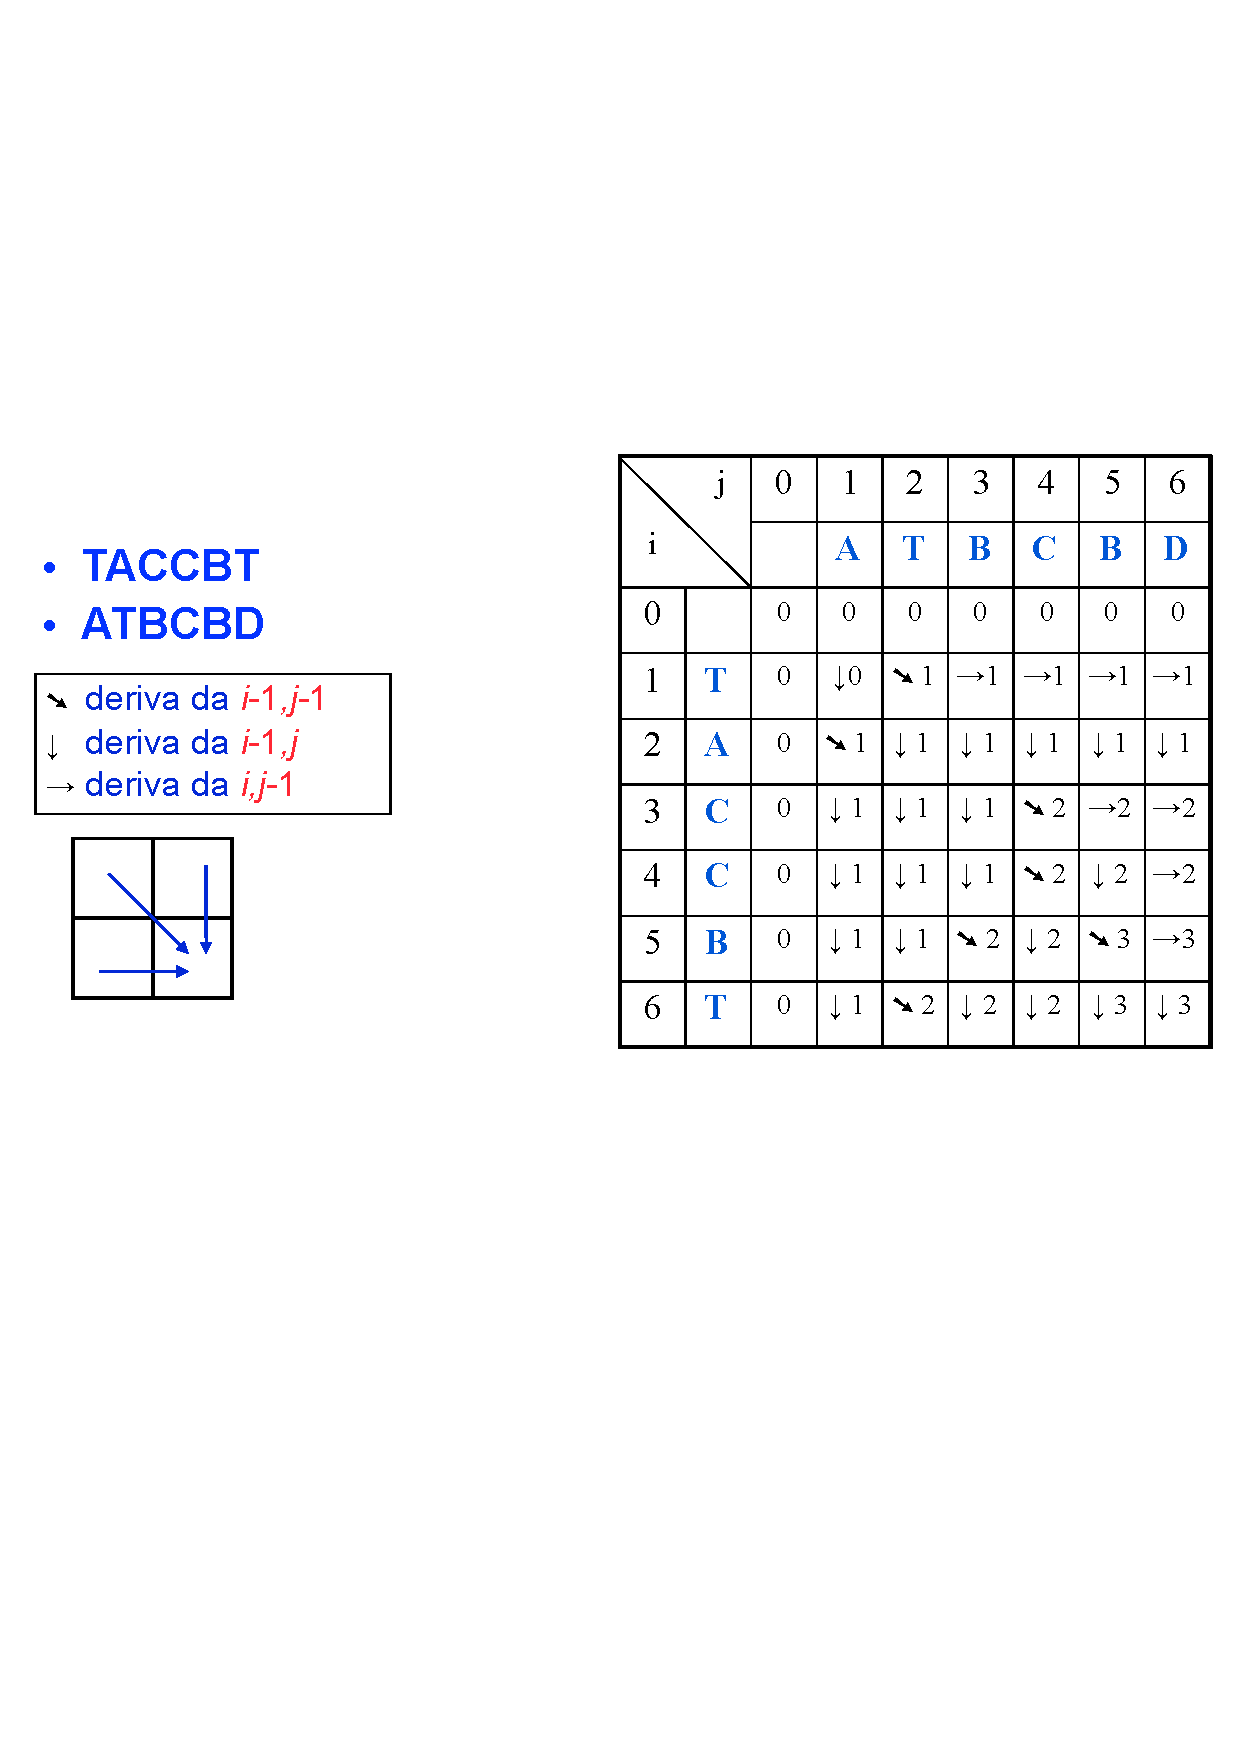
\includegraphics[width=0.95\textwidth,page=1]{lcs.pdf}

\tiny
\[
  \mathit{DP}(i,j) = \begin{cases}
   0 & i=0\ \OR\ j=0 \\
   \mathit{DP}(i-1,j-1)+1 & i>0\ \AND\ j>0\ \AND\ t_i = u_j \\
   \max \{ \mathit{DP}(i-1,j), \mathit{DP}(i,j-1) \} & i>0\ \AND\ j>0\ \AND\ t_i \neq u_j
  \end{cases}
\]

\end{frame}

% -----------------------------------------------------------------------------
\begin{frame}{Ricostruire la soluzione}

\centering
\vspace{-9pt}
\includegraphics[width=0.95\textwidth,page=2]{lcs.pdf}

\bigskip
\BB{Utilizzando la tabella, come possiamo ottenere la soluzione?}

\end{frame}


% -----------------------------------------------------------------------------
\begin{frame}[shrink=10]{Ricostruire la sottosequenza comune}

\vspace{-9pt}
\begin{Procedure}
\caption[A]{\INTEGER \LCS($\Item[\,]\ T,\ \Item[\,]\ U,\ \INTEGER\ n,\ \INTEGER\ m$)}
  $\ldots$\;
  \Return $\textsf{subsequence}(\mathit{DP}, T, U, n, m)$\;
\end{Procedure}

\vspace{-18pt}
\begin{Procedure}
\caption[A]{\textsf{subsequence}($\INTEGER[\,][\,]\ \mathit{DP}, \Item[\,]\ T,\ \Item[\,]\ U,\ \INTEGER\ i,\ \INTEGER\ j$)}
\If{$i \Eq 0$ \OR\ $j \Eq 0$}{
  \Return $\listconstructor()\;$
}
\eIf{$T[i] \Eq U[j]$}{
  $S = \textsf{subsequence}(\mathit{DP}, T, U, i-1, j-1)$\;
  $S.\listinsert(S.\listhead(), T[i])$\;
  \Return $S$\;
}{
  \eIf{$\mathit{DP}[i-1][j] > \mathit{DP}[i][j-1]$}{
    \Return $\textsf{subsequence}(\mathit{DP}, T, U, i-1, j)$\;
  }{
    \Return $\textsf{subsequence}(\mathit{DP}, T, U, i, j-1)$\;
  }
}
\end{Procedure}


\end{frame}

\begin{frame}{Complessità computazionale}

\vspace{-9pt}
\BB{Qual è la complessità computazionale di \textsf{subsequence()}?}

\pause
\[
  T(n) = O(m+n)
\]
  
\bigskip
\BB{Qual è la complessità computazionale di \textsf{LCS()}?}

\pause
\[
  T(n) = O(mn)
\]

\end{frame}

\begin{frame}{Commenti finali}

\vspace{-9pt}
\begin{myboxtitle}[Take-home message (prendi e porta a casa)]
Non sempre è necessario memorizzare informazioni aggiuntive per ricostruire la soluzione.
\end{myboxtitle}

\end{frame}

\begin{frame}{Reality check -- LCS e \texttt{diff}  }

\vspace{-9pt}
\BB{\texttt{diff}}
\BIL
\item Esamina due file di testo, evidenziondone le differenze a livello di riga. 
\item Lavorare \alert{a livello di riga} significa che i confronti fra simboli sono in realtà confronti fra righe, e che $n$ ed $m$ sono il numero di righe dei due file
\EIL

\BB{Ottimizzazioni}
\BIL
\item \texttt{diff} è utilizzato soprattutto per codice sorgente; è possibile applicare euristiche sulle righe iniziali e finali
\item Per distinguere le righe - utilizzo di funzioni hash
\EIL

\end{frame}

\begin{frame}{Reality check -- LCS e \texttt{diff}  }

\vspace{-9pt}
\IG{1.0}{diff.pdf}

\end{frame}


\end{document}



